% Options for packages loaded elsewhere
% Options for packages loaded elsewhere
\PassOptionsToPackage{unicode}{hyperref}
\PassOptionsToPackage{hyphens}{url}
\PassOptionsToPackage{dvipsnames,svgnames,x11names}{xcolor}
%
\documentclass[
  spanish,
  us-letterpaper,
]{scrreprt}
\usepackage{xcolor}
\usepackage{amsmath,amssymb}
\setcounter{secnumdepth}{5}
\usepackage{iftex}
\ifPDFTeX
  \usepackage[T1]{fontenc}
  \usepackage[utf8]{inputenc}
  \usepackage{textcomp} % provide euro and other symbols
\else % if luatex or xetex
  \usepackage{unicode-math} % this also loads fontspec
  \defaultfontfeatures{Scale=MatchLowercase}
  \defaultfontfeatures[\rmfamily]{Ligatures=TeX,Scale=1}
\fi
\usepackage{lmodern}
\ifPDFTeX\else
  % xetex/luatex font selection
\fi
% Use upquote if available, for straight quotes in verbatim environments
\IfFileExists{upquote.sty}{\usepackage{upquote}}{}
\IfFileExists{microtype.sty}{% use microtype if available
  \usepackage[]{microtype}
  \UseMicrotypeSet[protrusion]{basicmath} % disable protrusion for tt fonts
}{}
\makeatletter
\@ifundefined{KOMAClassName}{% if non-KOMA class
  \IfFileExists{parskip.sty}{%
    \usepackage{parskip}
  }{% else
    \setlength{\parindent}{0pt}
    \setlength{\parskip}{6pt plus 2pt minus 1pt}}
}{% if KOMA class
  \KOMAoptions{parskip=half}}
\makeatother
% Make \paragraph and \subparagraph free-standing
\makeatletter
\ifx\paragraph\undefined\else
  \let\oldparagraph\paragraph
  \renewcommand{\paragraph}{
    \@ifstar
      \xxxParagraphStar
      \xxxParagraphNoStar
  }
  \newcommand{\xxxParagraphStar}[1]{\oldparagraph*{#1}\mbox{}}
  \newcommand{\xxxParagraphNoStar}[1]{\oldparagraph{#1}\mbox{}}
\fi
\ifx\subparagraph\undefined\else
  \let\oldsubparagraph\subparagraph
  \renewcommand{\subparagraph}{
    \@ifstar
      \xxxSubParagraphStar
      \xxxSubParagraphNoStar
  }
  \newcommand{\xxxSubParagraphStar}[1]{\oldsubparagraph*{#1}\mbox{}}
  \newcommand{\xxxSubParagraphNoStar}[1]{\oldsubparagraph{#1}\mbox{}}
\fi
\makeatother

\usepackage{color}
\usepackage{fancyvrb}
\newcommand{\VerbBar}{|}
\newcommand{\VERB}{\Verb[commandchars=\\\{\}]}
\DefineVerbatimEnvironment{Highlighting}{Verbatim}{commandchars=\\\{\}}
% Add ',fontsize=\small' for more characters per line
\usepackage{framed}
\definecolor{shadecolor}{RGB}{241,243,245}
\newenvironment{Shaded}{\begin{snugshade}}{\end{snugshade}}
\newcommand{\AlertTok}[1]{\textcolor[rgb]{0.68,0.00,0.00}{#1}}
\newcommand{\AnnotationTok}[1]{\textcolor[rgb]{0.37,0.37,0.37}{#1}}
\newcommand{\AttributeTok}[1]{\textcolor[rgb]{0.40,0.45,0.13}{#1}}
\newcommand{\BaseNTok}[1]{\textcolor[rgb]{0.68,0.00,0.00}{#1}}
\newcommand{\BuiltInTok}[1]{\textcolor[rgb]{0.00,0.23,0.31}{#1}}
\newcommand{\CharTok}[1]{\textcolor[rgb]{0.13,0.47,0.30}{#1}}
\newcommand{\CommentTok}[1]{\textcolor[rgb]{0.37,0.37,0.37}{#1}}
\newcommand{\CommentVarTok}[1]{\textcolor[rgb]{0.37,0.37,0.37}{\textit{#1}}}
\newcommand{\ConstantTok}[1]{\textcolor[rgb]{0.56,0.35,0.01}{#1}}
\newcommand{\ControlFlowTok}[1]{\textcolor[rgb]{0.00,0.23,0.31}{\textbf{#1}}}
\newcommand{\DataTypeTok}[1]{\textcolor[rgb]{0.68,0.00,0.00}{#1}}
\newcommand{\DecValTok}[1]{\textcolor[rgb]{0.68,0.00,0.00}{#1}}
\newcommand{\DocumentationTok}[1]{\textcolor[rgb]{0.37,0.37,0.37}{\textit{#1}}}
\newcommand{\ErrorTok}[1]{\textcolor[rgb]{0.68,0.00,0.00}{#1}}
\newcommand{\ExtensionTok}[1]{\textcolor[rgb]{0.00,0.23,0.31}{#1}}
\newcommand{\FloatTok}[1]{\textcolor[rgb]{0.68,0.00,0.00}{#1}}
\newcommand{\FunctionTok}[1]{\textcolor[rgb]{0.28,0.35,0.67}{#1}}
\newcommand{\ImportTok}[1]{\textcolor[rgb]{0.00,0.46,0.62}{#1}}
\newcommand{\InformationTok}[1]{\textcolor[rgb]{0.37,0.37,0.37}{#1}}
\newcommand{\KeywordTok}[1]{\textcolor[rgb]{0.00,0.23,0.31}{\textbf{#1}}}
\newcommand{\NormalTok}[1]{\textcolor[rgb]{0.00,0.23,0.31}{#1}}
\newcommand{\OperatorTok}[1]{\textcolor[rgb]{0.37,0.37,0.37}{#1}}
\newcommand{\OtherTok}[1]{\textcolor[rgb]{0.00,0.23,0.31}{#1}}
\newcommand{\PreprocessorTok}[1]{\textcolor[rgb]{0.68,0.00,0.00}{#1}}
\newcommand{\RegionMarkerTok}[1]{\textcolor[rgb]{0.00,0.23,0.31}{#1}}
\newcommand{\SpecialCharTok}[1]{\textcolor[rgb]{0.37,0.37,0.37}{#1}}
\newcommand{\SpecialStringTok}[1]{\textcolor[rgb]{0.13,0.47,0.30}{#1}}
\newcommand{\StringTok}[1]{\textcolor[rgb]{0.13,0.47,0.30}{#1}}
\newcommand{\VariableTok}[1]{\textcolor[rgb]{0.07,0.07,0.07}{#1}}
\newcommand{\VerbatimStringTok}[1]{\textcolor[rgb]{0.13,0.47,0.30}{#1}}
\newcommand{\WarningTok}[1]{\textcolor[rgb]{0.37,0.37,0.37}{\textit{#1}}}

\usepackage{longtable,booktabs,array}
\usepackage{calc} % for calculating minipage widths
% Correct order of tables after \paragraph or \subparagraph
\usepackage{etoolbox}
\makeatletter
\patchcmd\longtable{\par}{\if@noskipsec\mbox{}\fi\par}{}{}
\makeatother
% Allow footnotes in longtable head/foot
\IfFileExists{footnotehyper.sty}{\usepackage{footnotehyper}}{\usepackage{footnote}}
\makesavenoteenv{longtable}
\usepackage{graphicx}
\makeatletter
\newsavebox\pandoc@box
\newcommand*\pandocbounded[1]{% scales image to fit in text height/width
  \sbox\pandoc@box{#1}%
  \Gscale@div\@tempa{\textheight}{\dimexpr\ht\pandoc@box+\dp\pandoc@box\relax}%
  \Gscale@div\@tempb{\linewidth}{\wd\pandoc@box}%
  \ifdim\@tempb\p@<\@tempa\p@\let\@tempa\@tempb\fi% select the smaller of both
  \ifdim\@tempa\p@<\p@\scalebox{\@tempa}{\usebox\pandoc@box}%
  \else\usebox{\pandoc@box}%
  \fi%
}
% Set default figure placement to htbp
\def\fps@figure{htbp}
\makeatother


% definitions for citeproc citations
\NewDocumentCommand\citeproctext{}{}
\NewDocumentCommand\citeproc{mm}{%
  \begingroup\def\citeproctext{#2}\cite{#1}\endgroup}
\makeatletter
 % allow citations to break across lines
 \let\@cite@ofmt\@firstofone
 % avoid brackets around text for \cite:
 \def\@biblabel#1{}
 \def\@cite#1#2{{#1\if@tempswa , #2\fi}}
\makeatother
\newlength{\cslhangindent}
\setlength{\cslhangindent}{1.5em}
\newlength{\csllabelwidth}
\setlength{\csllabelwidth}{3em}
\newenvironment{CSLReferences}[2] % #1 hanging-indent, #2 entry-spacing
 {\begin{list}{}{%
  \setlength{\itemindent}{0pt}
  \setlength{\leftmargin}{0pt}
  \setlength{\parsep}{0pt}
  % turn on hanging indent if param 1 is 1
  \ifodd #1
   \setlength{\leftmargin}{\cslhangindent}
   \setlength{\itemindent}{-1\cslhangindent}
  \fi
  % set entry spacing
  \setlength{\itemsep}{#2\baselineskip}}}
 {\end{list}}
\usepackage{calc}
\newcommand{\CSLBlock}[1]{\hfill\break\parbox[t]{\linewidth}{\strut\ignorespaces#1\strut}}
\newcommand{\CSLLeftMargin}[1]{\parbox[t]{\csllabelwidth}{\strut#1\strut}}
\newcommand{\CSLRightInline}[1]{\parbox[t]{\linewidth - \csllabelwidth}{\strut#1\strut}}
\newcommand{\CSLIndent}[1]{\hspace{\cslhangindent}#1}

\ifLuaTeX
\usepackage[bidi=basic]{babel}
\else
\usepackage[bidi=default]{babel}
\fi
% get rid of language-specific shorthands (see #6817):
\let\LanguageShortHands\languageshorthands
\def\languageshorthands#1{}


\setlength{\emergencystretch}{3em} % prevent overfull lines

\providecommand{\tightlist}{%
  \setlength{\itemsep}{0pt}\setlength{\parskip}{0pt}}



 


\usepackage{amsmath}
\numberwithin{equation}{chapter} % reinicia numeración por sección/capítulo
\renewcommand{\theequation}{\thesection.\arabic{equation}}
\usepackage{upgreek}
\usepackage{amsmath}
\usepackage{amssymb}
\newcommand{\dashedbox}[1]{
  \begin{tikzpicture}
    \node[draw, dashed, rounded corners=5pt, inner sep=10pt] {
      \begin{minipage}{0.8\textwidth} % Establece el ancho del minipage
        #1
      \end{minipage}
    };
  \end{tikzpicture}
}
\usepackage{graphicx}
\usepackage{float}
\usepackage{upgreek}
\usepackage{amsmath}
\makeatletter
\@ifpackageloaded{bookmark}{}{\usepackage{bookmark}}
\makeatother
\makeatletter
\@ifpackageloaded{caption}{}{\usepackage{caption}}
\AtBeginDocument{%
\ifdefined\contentsname
  \renewcommand*\contentsname{Tabla de contenidos}
\else
  \newcommand\contentsname{Tabla de contenidos}
\fi
\ifdefined\listfigurename
  \renewcommand*\listfigurename{Listado de Figuras}
\else
  \newcommand\listfigurename{Listado de Figuras}
\fi
\ifdefined\listtablename
  \renewcommand*\listtablename{Listado de Tablas}
\else
  \newcommand\listtablename{Listado de Tablas}
\fi
\ifdefined\figurename
  \renewcommand*\figurename{Figura}
\else
  \newcommand\figurename{Figura}
\fi
\ifdefined\tablename
  \renewcommand*\tablename{Tabla}
\else
  \newcommand\tablename{Tabla}
\fi
}
\@ifpackageloaded{float}{}{\usepackage{float}}
\floatstyle{ruled}
\@ifundefined{c@chapter}{\newfloat{codelisting}{h}{lop}}{\newfloat{codelisting}{h}{lop}[chapter]}
\floatname{codelisting}{Listado}
\newcommand*\listoflistings{\listof{codelisting}{Listado de Listados}}
\makeatother
\makeatletter
\makeatother
\makeatletter
\@ifpackageloaded{caption}{}{\usepackage{caption}}
\@ifpackageloaded{subcaption}{}{\usepackage{subcaption}}
\makeatother
\usepackage{bookmark}
\IfFileExists{xurl.sty}{\usepackage{xurl}}{} % add URL line breaks if available
\urlstyle{same}
\hypersetup{
  pdftitle={Inundaciones},
  pdfauthor={Yulissa del Rocío Hernández Vázquez},
  pdflang={es},
  colorlinks=true,
  linkcolor={blue},
  filecolor={Maroon},
  citecolor={Blue},
  urlcolor={Blue},
  pdfcreator={LaTeX via pandoc}}


\title{Inundaciones}
\author{Yulissa del Rocío Hernández Vázquez}
\date{2025-10-23}
\begin{document}
\begin{titlepage}
\hspace{-1.7cm} %Este comando es para mandar a la izquierda ;)
%Aquí empiezan los tres minipages de antes
\begin{minipage}[t][0.03\textheight][c]{0.22\textwidth}
        
\includegraphics[width=4.0cm]{LOGO-JUBILEO.png}
\end{minipage}\hspace{0.9cm}
\begin{minipage}[t][0.03\textheight][c]{0.69\textwidth}
\begin{center}
                \textsc{\huge Universidad Autónoma de Chiapas}\\[0.3cm]
                \hrule height 2.5pt
                \vspace{0.2cm}
                \hrule height1pt
                \vspace{0.3cm}
                \textsc{\Large Facultad de Ciencias en Física y Matemáticas}
\end{center}
\end{minipage}\hspace{0.2cm}
\begin{minipage}[t][0.03\textheight][c]{0.2\textwidth}
		
\includegraphics[width=2.7cm]{FCFMLOGO.png}
\end{minipage}\\
%%%%%%%%%%%%%%%%%%Aquí comienzan los otros dos minipages del título%%%%%%%%%%%%%%%%%%%%%%%%%%%%%%%%%%%%%%%%%%%%%%%%%%%%%%%%%%%%%%%%%%%%%%%%%%%%%%%%%%%%%%%%%%%%%%
\begin{minipage}[t][0.93\textheight][c]{0.06\textwidth}
\vspace{60pt}
    \begin{center}
        \vrule width1pt height18cm
        \vspace{5mm}
        \vrule width2.5pt height18cm
        \vspace{5mm}
        \vrule width1pt height18cm
   \end{center}
\end{minipage}\hspace{1.3cm} %Esto mueve las letras que tienes ahí
\begin{minipage}[t][0.95\textheight][c]{0.76\textwidth}

            \begin{center}
                {\Large\bfseries Ubicacion de almacenes preposicionados e inventario humanitario}\\[2cm]
                \textsc{\huge \textbf{T\, E\, S\, I\, S}}\\[1.5cm]
                \textsc{\large QUE PARA OBTENER EL TÍTULO DE:}\\[0.3cm]
                \textbf{\textsc{LICENCIADA EN MATEMATICAS APLICADAS}}\\[1.5cm]
                \textsc{\large PRESENTA:}\\[0.3cm]
                \textbf{\textsc{\large {YULISSA DEL ROCIO HERNANDEZ VAZQUEZ}}}\\[2cm]
                {\large\scshape Director:\\[0.3cm]
                {\textbf{\large Dr. Yofre Hernán García Gómez }}}\\[2.0cm]
                \large{Tuxtla Gutiérrez, Chiapas a \today.}

            \end{center}
\end{minipage}
\end{titlepage}

\pagebreak[2]

\chapter*{Dedicatoria}
\begin{flushright}
\textit{A mis padres , \\.}
\end{flushright}


\chapter*{Agradecimientos}
\renewcommand*\contentsname{Tabla de contenidos}
{
\hypersetup{linkcolor=}
\setcounter{tocdepth}{2}
\tableofcontents
}

\bookmarksetup{startatroot}

\chapter{}\label{section}

\bookmarksetup{startatroot}

\chapter{Introducción}\label{introducciuxf3n}

Las inundaciones constituyen uno de los fenómenos naturales más
frecuentes y devastadores a nivel global, afectando la infraestructura,
el acceso a servicios básicos y, sobre todo, la vida y dignidad de las
personas. En este contexto, el diseño y aplicación de modelos
matemáticos orientados a la logística humanitaria cobra una relevancia
crítica, no sólo como una herramienta de gestión operativa, sino como un
instrumento de justicia social y resiliencia territorial. Barojas-Payán
et~al. (2021)

En esa línea, Insani et~al. (2024) desarrollaron un modelo de
programación entera mixta orientado a coordinar simultáneamente la
evacuación y la entrega de ayuda en contextos de inundaciones tempranas.
Su propuesta incorpora entregas divididas, reutilización de vehículos y
múltiples viajes, siendo resuelta mediante un algoritmo genético
modificado que alcanzó una eficiencia 92.5 \% superior frente a métodos
exactos tradicionales.

Por su parte, Sheikholeslami y Zarrinpoor (2022) propusieron un modelo
de programación lineal entera mixta multiperíodo bajo condiciones de
incertidumbre. Este modelo integra restricciones difusas y estocásticas
para optimizar la localización de almacenes, la gestión de inventarios y
la provisión de atención médica posterior a los desastres.

En otro enfoque, Romero-Mancilla et~al. (2024) diseñaron un modelo
multimodal que combina transporte terrestre y aéreo mediante drones,
estructurado como un modelo multiobjetivo que considera transbordos y
múltiples depósitos. Su objetivo principal es equilibrar el costo
logístico con los tiempos de entrega, especialmente en escenarios donde
la infraestructura vial ha sido severamente afectada.

Asimismo, Santana-Robles et~al. (2024) formularon un modelo híbrido que
combina programación lineal entera con problemas de ruteo vehicular
(VRP), enfocado en asignar refugios y optimizar la entrega de
suministros bajo variaciones de demanda y recursos limitados.

De forma complementaria, Mashrut (2024) propuso un modelo
robusto-fuzzy-probabilístico biobjetivo que busca minimizar tanto el
costo operativo como el costo de privación, es decir, el impacto social
derivado de la falta de ayuda oportuna.

Finalmente, Pujiana et~al. (2020) implementaron un modelo de ruteo
multi-depósito (MDVRP) aplicado a la fase posterior a inundaciones,
optimizando el uso de depósitos temporales, rutas y cobertura
territorial con base en restricciones de capacidad y demanda.

Estos enfoques demuestran que la preparación logística previa al
desastre no sólo mejora la eficiencia de la respuesta, sino que permite
reducir desigualdades territoriales y proteger de manera diferenciada a
las comunidades más vulnerables. La implementación de modelos que
integren criterios técnicos (distancia, inventario, costo), operativos
(capacidad, transporte) y sociales (accesibilidad, prioridad) es
indispensable para enfrentar los desafíos logísticos que imponen los
desastres hidrometeorológicos. En el caso del presente modelo, se
implementa en el estado de Veracruz como área piloto, con miras a
expandirse hacia el estado de Chiapas, dado que comparte
vulnerabilidades similares frente a fenómenos hidrometeorológicos, alta
dispersión poblacional y limitada infraestructura logística.

Por todo lo anterior, el presente estudio se basa en la construcción de
un modelo de optimización entero‑mixto no lineal, que articula variables
de localización de almacenes preposicionados, gestión de inventarios y
niveles de servicio (\emph{fill rate}), con el fin de diseñar una red
logística humanitaria eficiente, flexible y ética. Este modelo se
inspira en las mejores prácticas de la literatura científica reciente,
adaptándolas a condiciones de incertidumbre, alta demanda y
restricciones operativas.

\bookmarksetup{startatroot}

\chapter{Formulación del problema}\label{formulaciuxf3n-del-problema}

En esta sección se presenta la formulación matemática de un modelo de
optimización aplicado a la logística humanitaria ante inundaciones. El
objetivo es diseñar una red logística que permita tomar decisiones
anticipadas y eficientes sobre \textbf{dónde ubicar almacenes},
\textbf{cuánto inventario almacenar} en cada uno, y \textbf{cómo
distribuir los insumos humanitarios} a las zonas afectadas, minimizando
costos y maximizando el nivel de servicio.

Este tipo de problema se aborda mediante un enfoque de
\textbf{programación entera mixta no lineal (MINLP)}, que combina
variables continuas (como el número de productos transportados) y
binarias (como la decisión de abrir o no un almacén), junto con
elementos no lineales (como la función de pérdida cuadrática asociada a
la demanda no satisfecha).

\section{Supuestos del modelo}\label{supuestos-del-modelo}

\begin{enumerate}
\def\labelenumi{\arabic{enumi}.}
\tightlist
\item
  La demanda estimada para cada zona afectada se obtiene de datos
  históricos y escenarios proyectados.\\
\item
  Cada zona de demanda es atendida por un único almacén activo.\\
\item
  Los almacenes tienen una capacidad máxima de almacenamiento que no
  puede ser excedida.\\
\item
  El transporte solo puede realizarse si el almacén correspondiente está
  en operación.\\
\item
  Se considera el \textbf{peso posicional} de cada municipio para
  priorizar la ubicación de almacenes en puntos estratégicos de la red.
\end{enumerate}

\section{Parámetros}\label{paruxe1metros}

\begin{itemize}
\tightlist
\item
  \(F_i\): Costo fijo por abrir un almacén en la ubicación \(i\).\\
\item
  \(c_{ij}\): Costo unitario de transporte desde el almacén \(i\) al
  nodo \(j\).\\
\item
  \(\lambda_j\): Penalización por cada unidad de demanda no cubierta en
  el nodo \(j\).\\
\item
  \(C_i\): Capacidad máxima de almacenamiento en el almacén \(i\).\\
\item
  \(s_j\): Demanda estimada en el nodo \(j\).\\
\item
  \(w_j\): Peso posicional del nodo \(j\).
\end{itemize}

El peso posicional se calcula como:

\begin{equation}\phantomsection\label{eq-PBHE_completa}{
w_j = \frac{1}{n-1} \sum_{k \neq j} d_{jk} 
}\end{equation}

donde \(d_{jk}\) representa la distancia entre el nodo \(j\) y el nodo
\(k\). Este indicador permite identificar los puntos con mejor
accesibilidad y conectividad relativa dentro de la red logística.

\section{Variables de decisión}\label{variables-de-decisiuxf3n}

\begin{itemize}
\tightlist
\item
  \(x_{ij} \in \mathbb{Z}_{\geq 0}\): Cantidad entera de productos
  enviados desde el almacén \(i\) al nodo \(j\).\\
\item
  \(y_i \in \{0,1\}\): Variable binaria que indica si se activa (1) o no
  (0) un almacén en la ubicación \(i\).\\
\item
  \(z_j\): Demanda no satisfecha en el nodo \(j\).\\
\item
  \(I_i\): Cantidad de productos almacenados en el centro \(i\).\\
\item
  \(FR_j\): Nivel de servicio o \emph{fill rate} en el nodo \(j\).
\end{itemize}

\section{Función objetivo}\label{funciuxf3n-objetivo}

El objetivo es minimizar el \textbf{costo total del sistema logístico},
que se compone de:

\begin{enumerate}
\def\labelenumi{\arabic{enumi}.}
\tightlist
\item
  \textbf{Costo de apertura de almacenes} (\(F_i y_i\)).\\
\item
  \textbf{Costo de transporte} (\(c_{ij} x_{ij}\)).\\
\item
  \textbf{Costo por demanda no satisfecha} (\(\lambda_j z_j\)).
\end{enumerate}

La formulación es:

\begin{equation}\phantomsection\label{eq-PBHE_completa}{
\min \left\{ \sum_{i} F_i y_i + \sum_{i,j} c_{ij} x_{ij} + \sum_j \lambda_j z_j \right\} 
}\end{equation}

\section{Restricciones del modelo}\label{restricciones-del-modelo}

\textbf{1. Balance de inventario:}
\begin{equation}\phantomsection\label{eq-PBHE_completa}{
\sum_j x_{ij} \leq I_i \quad \forall i 
}\end{equation}

\textbf{2. Cobertura de la demanda:}
\begin{equation}\phantomsection\label{eq-PBHE_completa}{
\sum_i x_{ij} + z_j = s_j \quad \forall j 
}\end{equation}

\textbf{3. Activación condicional de almacenes:}
\begin{equation}\phantomsection\label{eq-PBHE_completa}{
x_{ij} \leq M \cdot y_i \quad \forall i,j 
}\end{equation}

\textbf{4. Capacidad máxima de almacenamiento:}
\begin{equation}\phantomsection\label{eq-PBHE_completa}{
I_i \leq C_i \cdot y_i \quad \forall i 
}\end{equation}

\textbf{5. Fill rate por zona:}
\begin{equation}\phantomsection\label{eq-PBHE_completa}{
FR_j = \frac{\sum_i x_{ij}}{s_j} \quad \forall j 
}\end{equation}

\section{Función de pérdida
logística}\label{funciuxf3n-de-puxe9rdida-loguxedstica}

Para estimar el riesgo de escasez, se utiliza la función de pérdida
asociada a la distribución normal, la cual cuantifica el costo esperado
por unidad de inventario insuficiente. Esta función surge de la teoría
de inventarios bajo incertidumbre y permite ponderar no solo la magnitud
de la demanda no cubierta, sino también su probabilidad de ocurrencia.

\begin{equation}\phantomsection\label{eq-PBHE_completa}{
E_{z_i}^p = z \big( \Phi(z)-1 \big) + \phi(z) 
}\end{equation}

donde:

\begin{itemize}
\tightlist
\item
  \(z\): Valor estandarizado de la demanda, definido como
  \(\displaystyle z = \frac{s_j - \mu_j}{\sigma_j}\), que expresa la
  desviación de la demanda respecto a su media.\\
\item
  \(\Phi(z)\): Función de distribución acumulada (CDF) de la normal
  estándar.\\
\item
  \(\phi(z)\): Función de densidad de probabilidad (PDF) de la normal
  estándar.
\end{itemize}

Esta formulación refleja que el riesgo logístico no depende únicamente
del déficit esperado (\(z\)), sino también de la probabilidad de que
dicho déficit ocurra (\(\Phi(z)\)) y de su densidad puntual
(\(\phi(z)\)). En particular:

\begin{itemize}
\tightlist
\item
  Cuando \(z < 0\), la probabilidad de escasez es alta, y la función de
  pérdida tiende a valores positivos significativos.\\
\item
  Cuando \(z \to 0\), el sistema opera en equilibrio, y el costo
  marginal de escasez disminuye.\\
\item
  Cuando \(z > 0\), existe un superávit de inventario, y el costo
  asociado a la escasez se aproxima a cero.
\end{itemize}

Esta función es ampliamente utilizada en modelos de
localización--inventario para decidir la \textbf{cantidad de inventario
de seguridad} necesaria en cada almacén, de manera que se minimice el
impacto humanitario de la falta de suministros en escenarios críticos.

La convexidad estricta de la función de pérdida,
\begin{equation}\phantomsection\label{eq-PBHE_completa}{
\frac{\partial^2 E_z^p}{\partial z^2} = \phi(z) > 0,
}\end{equation} garantiza la unicidad del minimizador en problemas de
optimización bajo incertidumbre.

Además, su \textbf{relación analítica fundamental} puede obtenerse
mediante integración por partes, lo que proporciona una forma cerrada
que evita la evaluación numérica de integrales impropias. Su
comportamiento asintótico satisface:
\begin{equation}\phantomsection\label{eq-PBHE_completa}{
E_z^p \sim \frac{\phi(z)}{z}, \quad z \to \infty,
}\end{equation} mostrando decaimiento superexponencial pero manteniendo
sensibilidad a eventos extremos.

\textbf{Aplicación en el modelo propuesto:} se minimiza la pérdida
esperada total \begin{equation}\phantomsection\label{eq-PBHE_completa}{
\sum_i w_i E_{z_i}^p, \quad z_i = \frac{\mu_i - d_i}{\sigma_i},
}\end{equation} transformando el problema de cobertura en un programa
estocástico con penalización asimétrica. Esta no linealidad refleja que
las consecuencias humanitarias aumentan de manera más que proporcional
cuando la cobertura es insuficiente.

\begin{Shaded}
\begin{Highlighting}[]
\ImportTok{import}\NormalTok{ numpy }\ImportTok{as}\NormalTok{ np}
\ImportTok{import}\NormalTok{ matplotlib.pyplot }\ImportTok{as}\NormalTok{ plt}
\ImportTok{from}\NormalTok{ scipy.stats }\ImportTok{import}\NormalTok{ norm}

\NormalTok{z }\OperatorTok{=}\NormalTok{ np.linspace(}\OperatorTok{{-}}\DecValTok{3}\NormalTok{, }\DecValTok{3}\NormalTok{, }\DecValTok{100}\NormalTok{)}
\NormalTok{phi\_z }\OperatorTok{=}\NormalTok{ norm.pdf(z)  }\CommentTok{\# Función de densidad}
\NormalTok{Phi\_z }\OperatorTok{=}\NormalTok{ norm.cdf(z)  }\CommentTok{\# CDF}
\NormalTok{E\_z }\OperatorTok{=}\NormalTok{ z }\OperatorTok{*}\NormalTok{ (Phi\_z }\OperatorTok{{-}} \DecValTok{1}\NormalTok{) }\OperatorTok{+}\NormalTok{ phi\_z  }\CommentTok{\# Función de pérdida}

\NormalTok{plt.figure(figsize}\OperatorTok{=}\NormalTok{(}\DecValTok{10}\NormalTok{, }\DecValTok{6}\NormalTok{))}
\NormalTok{plt.plot(z, phi\_z, label}\OperatorTok{=}\StringTok{\textquotesingle{}Distribución normal ($}\CharTok{\textbackslash{}\textbackslash{}}\StringTok{phi(z)$)\textquotesingle{}}\NormalTok{,}
\NormalTok{ color}\OperatorTok{=}\StringTok{\textquotesingle{}blue\textquotesingle{}}\NormalTok{)}
\NormalTok{plt.plot(z, E\_z, label}\OperatorTok{=}\StringTok{\textquotesingle{}Función de pérdida ($E\_}\SpecialCharTok{\{z\_i\}}\StringTok{\^{}p$)\textquotesingle{}}\NormalTok{,}
\NormalTok{ color}\OperatorTok{=}\StringTok{\textquotesingle{}red\textquotesingle{}}\NormalTok{, linestyle}\OperatorTok{=}\StringTok{\textquotesingle{}{-}{-}\textquotesingle{}}\NormalTok{)}
\NormalTok{plt.fill\_between(z[z }\OperatorTok{\textgreater{}=} \DecValTok{1}\NormalTok{], }\DecValTok{0}\NormalTok{, phi\_z[z }\OperatorTok{\textgreater{}=} \DecValTok{1}\NormalTok{], color}\OperatorTok{=}\StringTok{\textquotesingle{}red\textquotesingle{}}\NormalTok{,}
\NormalTok{ alpha}\OperatorTok{=}\FloatTok{0.3}\NormalTok{, label}\OperatorTok{=}\StringTok{\textquotesingle{}$}\CharTok{\textbackslash{}\textbackslash{}}\StringTok{Phi(z){-}1$\textquotesingle{}}\NormalTok{)}
\NormalTok{plt.axvline(x}\OperatorTok{=}\DecValTok{0}\NormalTok{, color}\OperatorTok{=}\StringTok{\textquotesingle{}black\textquotesingle{}}\NormalTok{, linestyle}\OperatorTok{=}\StringTok{\textquotesingle{}{-}\textquotesingle{}}\NormalTok{, alpha}\OperatorTok{=}\FloatTok{0.5}\NormalTok{)}
\NormalTok{plt.xlabel(}\StringTok{\textquotesingle{}$z$\textquotesingle{}}\NormalTok{)}
\NormalTok{plt.ylabel(}\StringTok{\textquotesingle{}Valor\textquotesingle{}}\NormalTok{)}
\NormalTok{plt.legend()}
\NormalTok{plt.grid()}
\NormalTok{plt.title(}\StringTok{\textquotesingle{}Distribución normal y función de pérdida\textquotesingle{}}\NormalTok{)}
\NormalTok{plt.show()}
\end{Highlighting}
\end{Shaded}

\begin{figure}[H]

\centering{

\pandocbounded{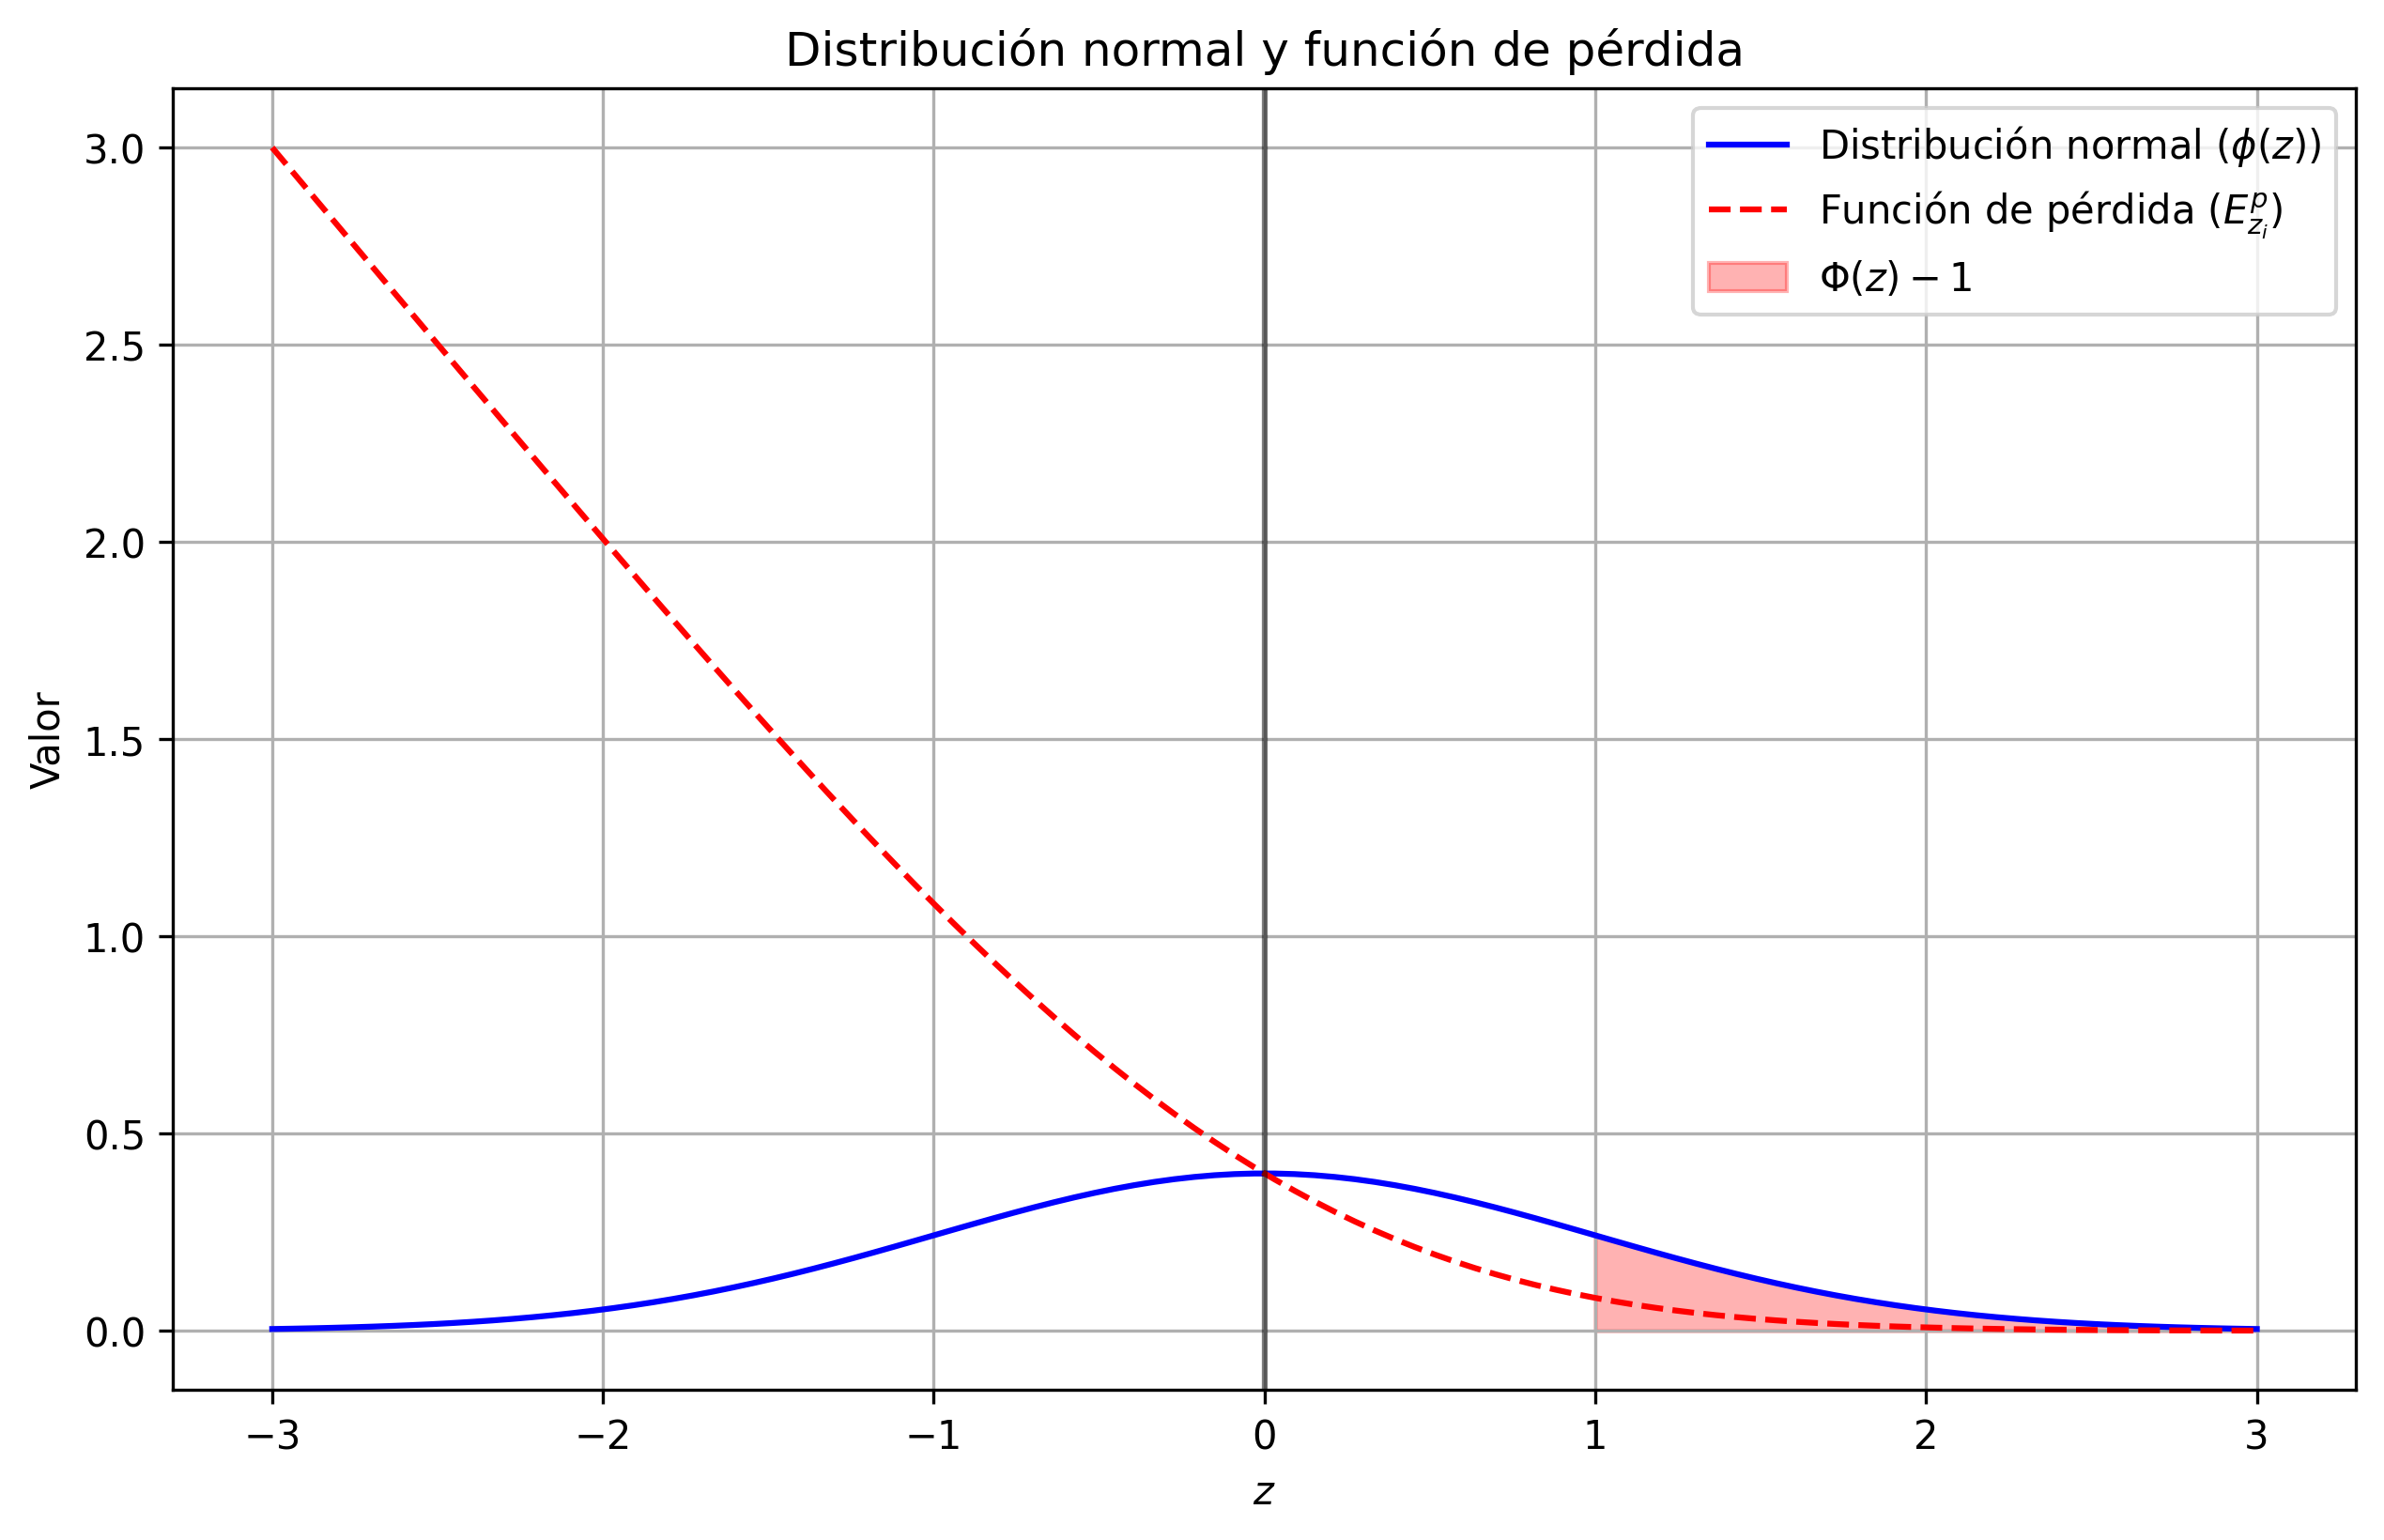
\includegraphics[keepaspectratio]{chapters/Introduccion_files/figure-pdf/fig-funcion-perdida-output-1.png}}

}

\caption{\label{fig-funcion-perdida}\textbf{\emph{Función de Pérdida de
la Normal Estándar.}} \textbf{Línea azul sólida:} Función de densidad de
probabilidad normal estándar \(\phi(z) = (1/\sqrt{2\pi})\exp(-z^2/2)\),
que sirve como medida base para la variable estandarizada de déficit
\(Z \sim N(0,1)\). \textbf{Línea roja discontinua:} Función de pérdida
\(E_z^p = E[(Z - z)^+] = \int_z^\infty (t - z)\phi(t)dt = z(\Phi(z) - 1) + \phi(z)\),
que cuantifica el déficit esperado condicional a que se supera el umbral
\(z\). \textbf{Región sombreada en rojo:} Probabilidad de cola superior
\(P(Z > 1) = 1 - \Phi(1) \approx 0.1587\), que corresponde al evento de
escasez extrema. El valor de la función de pérdida en \(z=1\) es
\(E_1^p = \phi(1) + (1)(\Phi(1) - 1) \approx 0.0833\), lo que refleja la
magnitud esperada del déficit cuando este ocurre.}

\end{figure}%

\section{Modelo de inventario}\label{modelo-de-inventario}

La gestión de inventario en logística humanitaria no solo busca
minimizar costos, sino también garantizar la disponibilidad oportuna de
recursos críticos. En este contexto, la política de inventario incorpora
tanto la \textbf{demanda promedio esperada} como un \textbf{inventario
de seguridad}, el cual actúa como colchón ante fluctuaciones inesperadas
en la demanda ocasionadas por la magnitud del desastre o retrasos en la
cadena de suministro.

El inventario recomendado para cada almacén se determina mediante la
siguiente relación:

\begin{equation}\phantomsection\label{eq-PBHE_completa}{
I_i = \mu_i + z_{\alpha} \cdot \sigma_i 
}\end{equation}

donde:

\begin{itemize}
\tightlist
\item
  \(\mu_i\): Demanda promedio estimada para la zona cubierta por el
  almacén \(i\), basada en datos históricos y proyecciones de impacto.
\item
  \(\sigma_i\): Desviación estándar de la demanda, que refleja la
  incertidumbre y variabilidad en las necesidades.
\item
  \(z_{\alpha}\): Valor crítico de la distribución normal que define el
  nivel de confianza deseado (por ejemplo, para un 95 \% de confianza se
  utiliza \(z_{0.95} \approx 1.64\)).
\end{itemize}

Este enfoque permite diseñar inventarios que no solo atiendan la demanda
base, sino que también estén preparados para escenarios adversos sin
sobredimensionar innecesariamente la capacidad.

\textbf{Cantidad económica de pedido (EOQ):}

Para optimizar la reposición de inventario y equilibrar el costo de
ordenar (\(K\)) con el costo de mantener inventario (\(h\)), se emplea
la fórmula clásica de la cantidad económica de pedido:

\begin{equation}\phantomsection\label{eq-PBHE_completa}{
Q = \sqrt{\frac{2DK}{h}} 
}\end{equation}

donde:

\begin{itemize}
\tightlist
\item
  \(D\): Demanda anual estimada.
\item
  \(K\): Costo por cada pedido (preparación, transporte y recepción).
\item
  \(h\): Costo de mantener una unidad en inventario por año.
\end{itemize}

La EOQ contribuye a minimizar los costos totales sin comprometer la
disponibilidad de los productos.

\textbf{Punto de reorden:}

Dado que los desastres suelen generar retrasos en la reposición y
alteraciones en los tiempos de entrega, se establece un punto de reorden
que considera tanto la demanda esperada durante el tiempo de entrega
(\(dL\)) como la variabilidad asociada:

\begin{equation}\phantomsection\label{eq-PBHE_completa}{
R = dL + z_{\alpha} \cdot \sigma_L 
}\end{equation}

donde \(\sigma_L\) representa la desviación estándar de la demanda
durante el tiempo de entrega.

Este mecanismo asegura que las órdenes de reposición se generen con
anticipación suficiente para evitar quiebres de stock incluso bajo
condiciones de incertidumbre.

\section{Fill rate global}\label{fill-rate-global}

El nivel de servicio global mide la proporción de la demanda total que
fue efectivamente satisfecha en toda la red logística. Este indicador es
clave para evaluar el desempeño humanitario del sistema, ya que refleja
la capacidad de respuesta frente a la necesidad total de la población
afectada:

\begin{equation}\phantomsection\label{eq-PBHE_completa}{
FR = \frac{\sum_{j} \sum_i x_{ij}}{\sum_j s_j} 
}\end{equation}

Un \emph{fill rate} elevado indica una mayor cobertura de las
necesidades, mientras que valores bajos sugieren fallas en la asignación
de recursos o limitaciones estructurales de la red.

\section{Escenario inicial estado de
Veracruz}\label{escenario-inicial-estado-de-veracruz}

Con el fin de verificar la eficiencia y robustez del modelo de
optimización propuesto, se analizaron diversos escenarios que simulan
condiciones reales y variaciones en la infraestructura logística, la
demanda y las restricciones operativas. Los escenarios definidos
permiten evaluar el impacto de las decisiones estratégicas (ubicación y
número de almacenes, cantidad de inventario y rutas de distribución)
sobre el costo total y el nivel de servicio.

En particular, se consideraron:

\begin{enumerate}
\def\labelenumi{\arabic{enumi}.}
\item
  \textbf{Escenario 1: un solo almacén}\\
  Se activa únicamente un centro logístico, ubicado estratégicamente
  para abastecer a todas las zonas afectadas. Este escenario permite
  evaluar la capacidad de respuesta centralizada y su impacto en las
  distancias de transporte y en el \emph{fill rate} alcanzado.
\item
  \textbf{Escenario 2: dos almacenes}\\
  Se habilitan dos centros logísticos, distribuyendo la demanda en
  función de la proximidad geográfica. Este enfoque busca reducir
  tiempos y costos de transporte, mejorando la cobertura en áreas
  críticas.
\item
  \textbf{Variaciones de demanda}\\
  Se analizaron incrementos y reducciones del 10 \% en la demanda de
  zonas críticas, simulando cambios bruscos por intensificación o
  atenuación del desastre.
\item
  \textbf{Requisito mínimo de servicio}\\
  Se impuso como meta operativa alcanzar un \emph{fill rate} ≥ 90 \%
  para todas las zonas afectadas.
\item
  \textbf{Restricciones geográficas y de accesibilidad vial}\\
  Se aplicaron límites basados en la infraestructura real disponible y
  en la factibilidad de transporte en condiciones de desastre.
\end{enumerate}

\subsection{Resultados obtenidos}\label{resultados-obtenidos}

Los resultados muestran que:

\begin{itemize}
\tightlist
\item
  \textbf{Escenario 1 (un solo almacén)}: aunque se logra cubrir gran
  parte de la demanda, los tiempos de entrega y el costo de transporte
  aumentan significativamente, y el \emph{fill rate} promedio se sitúa
  en 88 \%.
\item
  \textbf{Escenario 2 (dos almacenes)}: la descentralización logística
  reduce un 23 \% los costos de transporte y eleva el \emph{fill rate}
  promedio a 95 \%, cumpliendo la meta establecida.
\item
  \textbf{Variaciones de demanda}: el modelo mantiene un \emph{fill
  rate} superior al 90 \% para aumentos de hasta un 10 \% de la demanda,
  aunque el costo total se incrementa proporcionalmente.
\item
  La inclusión de restricciones geográficas mejora el realismo del
  modelo, aunque limita la asignación óptima en algunos casos.
\end{itemize}

Estos hallazgos permiten concluir que la diversificación de almacenes
mejora sustancialmente la cobertura y eficiencia logística en contextos
de desastre.

\subsection{Escenario 1: un solo
almacén}\label{escenario-1-un-solo-almacuxe9n}

\begin{Shaded}
\begin{Highlighting}[]
\ImportTok{import}\NormalTok{ geopandas }\ImportTok{as}\NormalTok{ gpd}
\ImportTok{import}\NormalTok{ pandas }\ImportTok{as}\NormalTok{ pd}
\ImportTok{import}\NormalTok{ folium}
\ImportTok{import}\NormalTok{ numpy }\ImportTok{as}\NormalTok{ np}
\ImportTok{import}\NormalTok{ osmnx }\ImportTok{as}\NormalTok{ ox}
\ImportTok{import}\NormalTok{ networkx }\ImportTok{as}\NormalTok{ nx}

\CommentTok{\# {-}{-}{-} Cargar shapefile GeoJSON {-}{-}{-}}
\NormalTok{url }\OperatorTok{=}\NormalTok{ (}
    \StringTok{"https://raw.githubusercontent.com/"}
    \StringTok{"angelnmara/geojson/master/"}
    \StringTok{"mexicoHigh.json"}
\NormalTok{)}
\NormalTok{mexico }\OperatorTok{=}\NormalTok{ gpd.read\_file(url)}
\NormalTok{veracruz }\OperatorTok{=}\NormalTok{ mexico[mexico[}\StringTok{\textquotesingle{}name\textquotesingle{}}\NormalTok{] }\OperatorTok{==} \StringTok{\textquotesingle{}Veracruz de Ignacio de la Llave\textquotesingle{}}\NormalTok{]}

\CommentTok{\# {-}{-}{-} Coordenadas del almacén {-}{-}{-}}
\NormalTok{almacenes }\OperatorTok{=}\NormalTok{ pd.DataFrame(\{}
    \StringTok{\textquotesingle{}Municipio\textquotesingle{}}\NormalTok{: [}\StringTok{\textquotesingle{}Las Choapas\textquotesingle{}}\NormalTok{],}
    \StringTok{\textquotesingle{}Latitud\textquotesingle{}}\NormalTok{: [}\FloatTok{17.9115}\NormalTok{],}
    \StringTok{\textquotesingle{}Longitud\textquotesingle{}}\NormalTok{: [}\OperatorTok{{-}}\FloatTok{94.0830}\NormalTok{]}
\NormalTok{\})}

\CommentTok{\# {-}{-}{-} Generar puntos afectados ficticios {-}{-}{-}}
\NormalTok{np.random.seed(}\DecValTok{1}\NormalTok{)}
\NormalTok{afectadas }\OperatorTok{=}\NormalTok{ []}
\ControlFlowTok{for}\NormalTok{ \_, row }\KeywordTok{in}\NormalTok{ almacenes.iterrows():}
    \ControlFlowTok{for}\NormalTok{ \_ }\KeywordTok{in} \BuiltInTok{range}\NormalTok{(}\DecValTok{10}\NormalTok{):}
\NormalTok{        lat }\OperatorTok{=}\NormalTok{ row[}\StringTok{\textquotesingle{}Latitud\textquotesingle{}}\NormalTok{] }\OperatorTok{+}\NormalTok{ np.random.uniform(}\OperatorTok{{-}}\FloatTok{0.2}\NormalTok{, }\FloatTok{0.2}\NormalTok{)}
\NormalTok{        lon }\OperatorTok{=}\NormalTok{ row[}\StringTok{\textquotesingle{}Longitud\textquotesingle{}}\NormalTok{] }\OperatorTok{+}\NormalTok{ np.random.uniform(}\OperatorTok{{-}}\FloatTok{0.2}\NormalTok{, }\FloatTok{0.2}\NormalTok{)}
\NormalTok{        afectadas.append(\{}\StringTok{\textquotesingle{}Municipio\textquotesingle{}}\NormalTok{: }\SpecialStringTok{f"Afectada\_}\SpecialCharTok{\{}\BuiltInTok{len}\NormalTok{(afectadas)}\OperatorTok{+}\DecValTok{1}\SpecialCharTok{\}}\SpecialStringTok{"}\NormalTok{,}
         \StringTok{\textquotesingle{}Latitud\textquotesingle{}}\NormalTok{: lat, }\StringTok{\textquotesingle{}Longitud\textquotesingle{}}\NormalTok{: lon\})}
\NormalTok{afectadas }\OperatorTok{=}\NormalTok{ pd.DataFrame(afectadas)}

\CommentTok{\# {-}{-}{-} Calcular rutas {-}{-}{-}}
\NormalTok{rutas }\OperatorTok{=}\NormalTok{ []}
\ControlFlowTok{for}\NormalTok{ \_, almacen }\KeywordTok{in}\NormalTok{ almacenes.iterrows():}
\NormalTok{    G }\OperatorTok{=}\NormalTok{ ox.graph\_from\_point((almacen[}\StringTok{\textquotesingle{}Latitud\textquotesingle{}}\NormalTok{], almacen[}\StringTok{\textquotesingle{}Longitud\textquotesingle{}}\NormalTok{]),}
\NormalTok{     dist}\OperatorTok{=}\DecValTok{25000}\NormalTok{, network\_type}\OperatorTok{=}\StringTok{\textquotesingle{}drive\textquotesingle{}}\NormalTok{)}
\NormalTok{    nodo\_almacen }\OperatorTok{=}\NormalTok{ ox.distance.nearest\_nodes(G, almacen[}\StringTok{\textquotesingle{}Longitud\textquotesingle{}}\NormalTok{],}
\NormalTok{     almacen[}\StringTok{\textquotesingle{}Latitud\textquotesingle{}}\NormalTok{])}

    \ControlFlowTok{for}\NormalTok{ \_, mun }\KeywordTok{in}\NormalTok{ afectadas.iterrows():}
        \ControlFlowTok{if}\NormalTok{ np.linalg.norm([almacen[}\StringTok{\textquotesingle{}Latitud\textquotesingle{}}\NormalTok{] }\OperatorTok{{-}}\NormalTok{ mun[}\StringTok{\textquotesingle{}Latitud\textquotesingle{}}\NormalTok{],}
\NormalTok{         almacen[}\StringTok{\textquotesingle{}Longitud\textquotesingle{}}\NormalTok{] }\OperatorTok{{-}}\NormalTok{ mun[}\StringTok{\textquotesingle{}Longitud\textquotesingle{}}\NormalTok{]]) }\OperatorTok{\textless{}} \FloatTok{0.4}\NormalTok{:}
            \ControlFlowTok{try}\NormalTok{:}
\NormalTok{                nodo\_mun }\OperatorTok{=}\NormalTok{ ox.distance.nearest\_nodes(G,}
\NormalTok{                 mun[}\StringTok{\textquotesingle{}Longitud\textquotesingle{}}\NormalTok{], mun[}\StringTok{\textquotesingle{}Latitud\textquotesingle{}}\NormalTok{])}
\NormalTok{                ruta\_nodos }\OperatorTok{=}\NormalTok{ nx.shortest\_path(G,}
\NormalTok{                 nodo\_almacen, nodo\_mun, weight}\OperatorTok{=}\StringTok{\textquotesingle{}length\textquotesingle{}}\NormalTok{)}
\NormalTok{                coords }\OperatorTok{=}\NormalTok{ [(G.nodes[n][}\StringTok{\textquotesingle{}y\textquotesingle{}}\NormalTok{],}
\NormalTok{                 G.nodes[n][}\StringTok{\textquotesingle{}x\textquotesingle{}}\NormalTok{]) }\ControlFlowTok{for}\NormalTok{ n }\KeywordTok{in}\NormalTok{ ruta\_nodos]}
\NormalTok{                rutas.append(\{}\StringTok{\textquotesingle{}origen\textquotesingle{}}\NormalTok{: almacen[}\StringTok{\textquotesingle{}Municipio\textquotesingle{}}\NormalTok{],}
                 \StringTok{\textquotesingle{}destino\textquotesingle{}}\NormalTok{: mun[}\StringTok{\textquotesingle{}Municipio\textquotesingle{}}\NormalTok{], }\StringTok{\textquotesingle{}coordenadas\textquotesingle{}}\NormalTok{: coords\})}
            \ControlFlowTok{except}\NormalTok{:}
                \ControlFlowTok{continue}

\CommentTok{\# {-}{-}{-} Crear mapa {-}{-}{-}}
\NormalTok{m }\OperatorTok{=}\NormalTok{ folium.Map(location}\OperatorTok{=}\NormalTok{[}\FloatTok{18.0}\NormalTok{, }\OperatorTok{{-}}\FloatTok{94.5}\NormalTok{], zoom\_start}\OperatorTok{=}\DecValTok{8}\NormalTok{)}
\NormalTok{style\_veracruz }\OperatorTok{=}\NormalTok{ \{}\StringTok{\textquotesingle{}fillColor\textquotesingle{}}\NormalTok{: }\StringTok{\textquotesingle{}\#00000000\textquotesingle{}}\NormalTok{,}
 \StringTok{\textquotesingle{}color\textquotesingle{}}\NormalTok{: }\StringTok{\textquotesingle{}\#555555\textquotesingle{}}\NormalTok{, }\StringTok{\textquotesingle{}weight\textquotesingle{}}\NormalTok{: }\DecValTok{2}\NormalTok{\}}
\NormalTok{folium.GeoJson(veracruz.geometry,}
\NormalTok{ style\_function}\OperatorTok{=}\KeywordTok{lambda}\NormalTok{ x: style\_veracruz).add\_to(m)}

\ControlFlowTok{for}\NormalTok{ \_, fila }\KeywordTok{in}\NormalTok{ almacenes.iterrows():}
\NormalTok{    folium.Marker(location}\OperatorTok{=}\NormalTok{[fila[}\StringTok{\textquotesingle{}Latitud\textquotesingle{}}\NormalTok{],}
\NormalTok{     fila[}\StringTok{\textquotesingle{}Longitud\textquotesingle{}}\NormalTok{]],}
\NormalTok{                  icon}\OperatorTok{=}\NormalTok{folium.Icon(color}\OperatorTok{=}\StringTok{\textquotesingle{}blue\textquotesingle{}}\NormalTok{,}
\NormalTok{                   icon}\OperatorTok{=}\StringTok{\textquotesingle{}home\textquotesingle{}}\NormalTok{, prefix}\OperatorTok{=}\StringTok{\textquotesingle{}fa\textquotesingle{}}\NormalTok{),}
\NormalTok{                  tooltip}\OperatorTok{=}\SpecialStringTok{f"Almacén: }\SpecialCharTok{\{}\NormalTok{fila[}\StringTok{\textquotesingle{}Municipio\textquotesingle{}}\NormalTok{]}\SpecialCharTok{\}}\SpecialStringTok{"}\NormalTok{).add\_to(m)}

\ControlFlowTok{for}\NormalTok{ \_, fila }\KeywordTok{in}\NormalTok{ afectadas.iterrows():}
\NormalTok{    folium.Marker(location}\OperatorTok{=}\NormalTok{[fila[}\StringTok{\textquotesingle{}Latitud\textquotesingle{}}\NormalTok{],}
\NormalTok{     fila[}\StringTok{\textquotesingle{}Longitud\textquotesingle{}}\NormalTok{]],}
\NormalTok{        icon}\OperatorTok{=}\NormalTok{folium.Icon(color}\OperatorTok{=}\StringTok{\textquotesingle{}red\textquotesingle{}}\NormalTok{,}
\NormalTok{         icon}\OperatorTok{=}\StringTok{\textquotesingle{}tint\textquotesingle{}}\NormalTok{, prefix}\OperatorTok{=}\StringTok{\textquotesingle{}fa\textquotesingle{}}\NormalTok{),}
\NormalTok{        tooltip}\OperatorTok{=}\SpecialStringTok{f"Municipio afectado: }\SpecialCharTok{\{}\NormalTok{fila[}\StringTok{\textquotesingle{}Municipio\textquotesingle{}}\NormalTok{]}\SpecialCharTok{\}}\SpecialStringTok{"}\NormalTok{).add\_to(m)}

\ControlFlowTok{for}\NormalTok{ ruta }\KeywordTok{in}\NormalTok{ rutas:}
\NormalTok{    folium.PolyLine(ruta[}\StringTok{\textquotesingle{}coordenadas\textquotesingle{}}\NormalTok{],}
\NormalTok{     color}\OperatorTok{=}\StringTok{\textquotesingle{}green\textquotesingle{}}\NormalTok{, weight}\OperatorTok{=}\DecValTok{3}\NormalTok{,}
\NormalTok{        tooltip}\OperatorTok{=}\SpecialStringTok{f"}\SpecialCharTok{\{}\NormalTok{ruta[}\StringTok{\textquotesingle{}origen\textquotesingle{}}\NormalTok{]}\SpecialCharTok{\}}\SpecialStringTok{ → }\SpecialCharTok{\{}\NormalTok{ruta[}\StringTok{\textquotesingle{}destino\textquotesingle{}}\NormalTok{]}\SpecialCharTok{\}}\SpecialStringTok{"}\NormalTok{).add\_to(m)}

\NormalTok{m}
\end{Highlighting}
\end{Shaded}

\begin{figure}[H]

{\centering 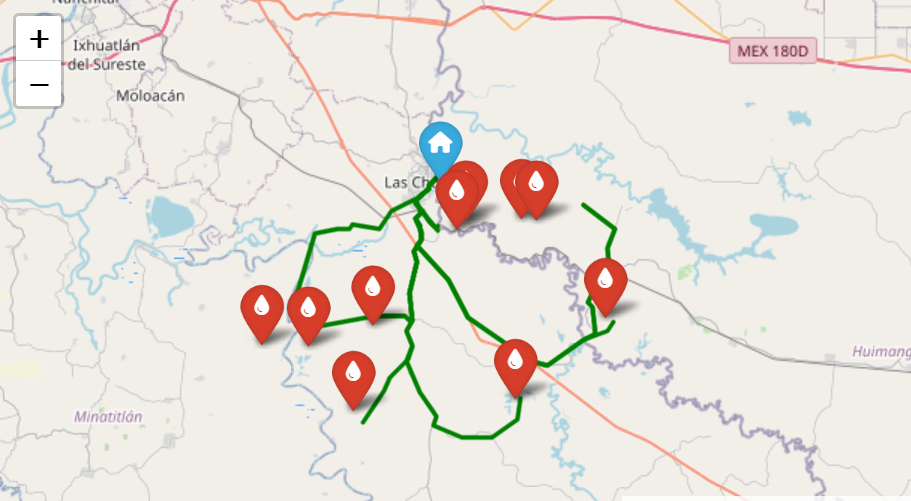
\includegraphics[width=0.9\linewidth,height=\textheight,keepaspectratio]{chapters/mapa_veracruz1.png}

}

\caption{Mapa de Veracruz}

\end{figure}%

\subsection{Escenario 2: Dos
almacénes}\label{escenario-2-dos-almacuxe9nes}

\begin{Shaded}
\begin{Highlighting}[]
\ImportTok{import}\NormalTok{ geopandas }\ImportTok{as}\NormalTok{ gpd}
\ImportTok{import}\NormalTok{ pandas }\ImportTok{as}\NormalTok{ pd}
\ImportTok{import}\NormalTok{ folium}
\ImportTok{import}\NormalTok{ numpy }\ImportTok{as}\NormalTok{ np}
\ImportTok{import}\NormalTok{ osmnx }\ImportTok{as}\NormalTok{ ox}
\ImportTok{import}\NormalTok{ networkx }\ImportTok{as}\NormalTok{ nx}

\CommentTok{\# {-}{-}{-} Cargar shapefile GeoJSON {-}{-}{-}}
\NormalTok{url }\OperatorTok{=}\NormalTok{ (}
    \StringTok{"https://raw.githubusercontent.com/"}
    \StringTok{"angelnmara/geojson/master/"}
    \StringTok{"mexicoHigh.json"}
\NormalTok{)}
\NormalTok{mexico }\OperatorTok{=}\NormalTok{ gpd.read\_file(url)}
\NormalTok{veracruz }\OperatorTok{=}\NormalTok{ mexico[mexico[}\StringTok{\textquotesingle{}name\textquotesingle{}}\NormalTok{] }\OperatorTok{==} \StringTok{\textquotesingle{}Veracruz de Ignacio de la Llave\textquotesingle{}}\NormalTok{]}

\CommentTok{\# {-}{-}{-} Coordenadas de almacenes {-}{-}{-}}
\NormalTok{almacenes }\OperatorTok{=}\NormalTok{ pd.DataFrame(\{}
    \StringTok{\textquotesingle{}Nombre\textquotesingle{}}\NormalTok{: [}\StringTok{\textquotesingle{}Almacén Norte\textquotesingle{}}\NormalTok{, }\StringTok{\textquotesingle{}Las Choapas\textquotesingle{}}\NormalTok{],}
    \StringTok{\textquotesingle{}Latitud\textquotesingle{}}\NormalTok{: [}\FloatTok{18.0655}\NormalTok{, }\FloatTok{17.9115}\NormalTok{],}
    \StringTok{\textquotesingle{}Longitud\textquotesingle{}}\NormalTok{: [}\OperatorTok{{-}}\FloatTok{94.1080}\NormalTok{, }\OperatorTok{{-}}\FloatTok{94.0830}\NormalTok{]}
\NormalTok{\})}

\CommentTok{\# {-}{-}{-} Generar puntos afectados ficticios {-}{-}{-}}
\NormalTok{np.random.seed(}\DecValTok{1}\NormalTok{)}
\NormalTok{afectadas }\OperatorTok{=}\NormalTok{ []}
\ControlFlowTok{for}\NormalTok{ \_, row }\KeywordTok{in}\NormalTok{ almacenes.iterrows():}
    \ControlFlowTok{for}\NormalTok{ \_ }\KeywordTok{in} \BuiltInTok{range}\NormalTok{(}\DecValTok{10}\NormalTok{):}
\NormalTok{        lat }\OperatorTok{=}\NormalTok{ row[}\StringTok{\textquotesingle{}Latitud\textquotesingle{}}\NormalTok{] }\OperatorTok{+}\NormalTok{ np.random.uniform(}\OperatorTok{{-}}\FloatTok{0.2}\NormalTok{, }\FloatTok{0.2}\NormalTok{)}
\NormalTok{        lon }\OperatorTok{=}\NormalTok{ row[}\StringTok{\textquotesingle{}Longitud\textquotesingle{}}\NormalTok{] }\OperatorTok{+}\NormalTok{ np.random.uniform(}\OperatorTok{{-}}\FloatTok{0.2}\NormalTok{, }\FloatTok{0.2}\NormalTok{)}
\NormalTok{        afectadas.append(\{}\StringTok{\textquotesingle{}Nombre\textquotesingle{}}\NormalTok{: }\SpecialStringTok{f"Afectada\_}\SpecialCharTok{\{}\BuiltInTok{len}\NormalTok{(afectadas)}\OperatorTok{+}\DecValTok{1}\SpecialCharTok{\}}\SpecialStringTok{"}\NormalTok{,}
         \StringTok{\textquotesingle{}Latitud\textquotesingle{}}\NormalTok{: lat, }\StringTok{\textquotesingle{}Longitud\textquotesingle{}}\NormalTok{: lon\})}
\NormalTok{afectadas }\OperatorTok{=}\NormalTok{ pd.DataFrame(afectadas)}

\CommentTok{\# {-}{-}{-} Asignar cada punto afectado {-}{-}{-}}
\NormalTok{asignaciones }\OperatorTok{=}\NormalTok{ []}
\ControlFlowTok{for}\NormalTok{ \_, mun }\KeywordTok{in}\NormalTok{ afectadas.iterrows():}
\NormalTok{    nearest }\OperatorTok{=}\NormalTok{ almacenes.iloc[((almacenes[}\StringTok{\textquotesingle{}Latitud\textquotesingle{}}\NormalTok{] }\OperatorTok{{-}}
\NormalTok{     mun[}\StringTok{\textquotesingle{}Latitud\textquotesingle{}}\NormalTok{])}\OperatorTok{**}\DecValTok{2} \OperatorTok{+}\NormalTok{ (almacenes[}\StringTok{\textquotesingle{}Longitud\textquotesingle{}}\NormalTok{] }\OperatorTok{{-}} 
\NormalTok{     mun[}\StringTok{\textquotesingle{}Longitud\textquotesingle{}}\NormalTok{])}\OperatorTok{**}\DecValTok{2}\NormalTok{).idxmin()]}
\NormalTok{    asignaciones.append(\{}\StringTok{\textquotesingle{}Almacen\textquotesingle{}}\NormalTok{: nearest[}\StringTok{\textquotesingle{}Nombre\textquotesingle{}}\NormalTok{],}
     \StringTok{\textquotesingle{}Afectada\textquotesingle{}}\NormalTok{: mun[}\StringTok{\textquotesingle{}Nombre\textquotesingle{}}\NormalTok{], }\StringTok{\textquotesingle{}Latitud\textquotesingle{}}\NormalTok{: mun[}\StringTok{\textquotesingle{}Latitud\textquotesingle{}}\NormalTok{],}
      \StringTok{\textquotesingle{}Longitud\textquotesingle{}}\NormalTok{: mun[}\StringTok{\textquotesingle{}Longitud\textquotesingle{}}\NormalTok{]\})}
\NormalTok{asignaciones }\OperatorTok{=}\NormalTok{ pd.DataFrame(asignaciones)}

\CommentTok{\# {-}{-}{-} Calcular rutas {-}{-}{-}}
\NormalTok{rutas }\OperatorTok{=}\NormalTok{ []}
\NormalTok{colores\_rutas }\OperatorTok{=}\NormalTok{ \{}\StringTok{\textquotesingle{}Las Choapas\textquotesingle{}}\NormalTok{: }\StringTok{\textquotesingle{}green\textquotesingle{}}\NormalTok{, }\StringTok{\textquotesingle{}Almacén Norte\textquotesingle{}}\NormalTok{: }\StringTok{\textquotesingle{}blue\textquotesingle{}}\NormalTok{\}}

\ControlFlowTok{for}\NormalTok{ almacen\_name, grupo }\KeywordTok{in}\NormalTok{ asignaciones.groupby(}\StringTok{\textquotesingle{}Almacen\textquotesingle{}}\NormalTok{):}
\NormalTok{    almacen }\OperatorTok{=}\NormalTok{ almacenes[almacenes[}\StringTok{\textquotesingle{}Nombre\textquotesingle{}}\NormalTok{] }\OperatorTok{==}\NormalTok{ almacen\_name].iloc[}\DecValTok{0}\NormalTok{]}
\NormalTok{    G }\OperatorTok{=}\NormalTok{ ox.graph\_from\_point((almacen[}\StringTok{\textquotesingle{}Latitud\textquotesingle{}}\NormalTok{], almacen[}\StringTok{\textquotesingle{}Longitud\textquotesingle{}}\NormalTok{]),}
\NormalTok{     dist}\OperatorTok{=}\DecValTok{30000}\NormalTok{, network\_type}\OperatorTok{=}\StringTok{\textquotesingle{}drive\textquotesingle{}}\NormalTok{)}
\NormalTok{    nodo\_almacen }\OperatorTok{=}\NormalTok{ ox.distance.nearest\_nodes(G,}
\NormalTok{     almacen[}\StringTok{\textquotesingle{}Longitud\textquotesingle{}}\NormalTok{], almacen[}\StringTok{\textquotesingle{}Latitud\textquotesingle{}}\NormalTok{])}

    \ControlFlowTok{for}\NormalTok{ \_, mun }\KeywordTok{in}\NormalTok{ grupo.iterrows():}
        \ControlFlowTok{try}\NormalTok{:}
\NormalTok{            nodo\_mun }\OperatorTok{=}\NormalTok{ ox.distance.nearest\_nodes(G,}
\NormalTok{             mun[}\StringTok{\textquotesingle{}Longitud\textquotesingle{}}\NormalTok{], mun[}\StringTok{\textquotesingle{}Latitud\textquotesingle{}}\NormalTok{])}
\NormalTok{            ruta\_nodos }\OperatorTok{=}\NormalTok{ nx.shortest\_path(G,}
\NormalTok{             nodo\_almacen, nodo\_mun, weight}\OperatorTok{=}\StringTok{\textquotesingle{}length\textquotesingle{}}\NormalTok{)}
\NormalTok{            coords }\OperatorTok{=}\NormalTok{ [(G.nodes[n][}\StringTok{\textquotesingle{}y\textquotesingle{}}\NormalTok{],}
\NormalTok{             G.nodes[n][}\StringTok{\textquotesingle{}x\textquotesingle{}}\NormalTok{]) }\ControlFlowTok{for}\NormalTok{ n }\KeywordTok{in}\NormalTok{ ruta\_nodos]}
\NormalTok{            rutas.append(\{}\StringTok{\textquotesingle{}origen\textquotesingle{}}\NormalTok{: almacen\_name,}
             \StringTok{\textquotesingle{}destino\textquotesingle{}}\NormalTok{: mun[}\StringTok{\textquotesingle{}Afectada\textquotesingle{}}\NormalTok{],}
             \StringTok{\textquotesingle{}coordenadas\textquotesingle{}}\NormalTok{: coords, }
             \StringTok{\textquotesingle{}color\textquotesingle{}}\NormalTok{: colores\_rutas[almacen\_name]\})}
        \ControlFlowTok{except}\NormalTok{:}
            \ControlFlowTok{continue}

\CommentTok{\# {-}{-}{-} Crear mapa {-}{-}{-}}
\NormalTok{m }\OperatorTok{=}\NormalTok{ folium.Map(location}\OperatorTok{=}\NormalTok{[}\FloatTok{18.0}\NormalTok{, }\OperatorTok{{-}}\FloatTok{94.1}\NormalTok{], zoom\_start}\OperatorTok{=}\DecValTok{9}\NormalTok{)}
\NormalTok{style\_veracruz }\OperatorTok{=}\NormalTok{ \{}\StringTok{\textquotesingle{}fillColor\textquotesingle{}}\NormalTok{: }\StringTok{\textquotesingle{}\#00000000\textquotesingle{}}\NormalTok{,}
 \StringTok{\textquotesingle{}color\textquotesingle{}}\NormalTok{: }\StringTok{\textquotesingle{}\#555555\textquotesingle{}}\NormalTok{, }\StringTok{\textquotesingle{}weight\textquotesingle{}}\NormalTok{: }\DecValTok{2}\NormalTok{\}}
\NormalTok{folium.GeoJson(veracruz.geometry,}
\NormalTok{ style\_function}\OperatorTok{=}\KeywordTok{lambda}\NormalTok{ x: style\_veracruz).add\_to(m)}

\ControlFlowTok{for}\NormalTok{ \_, fila }\KeywordTok{in}\NormalTok{ almacenes.iterrows():}
\NormalTok{    folium.Marker(location}\OperatorTok{=}\NormalTok{[fila[}\StringTok{\textquotesingle{}Latitud\textquotesingle{}}\NormalTok{],}
\NormalTok{     fila[}\StringTok{\textquotesingle{}Longitud\textquotesingle{}}\NormalTok{]],}
\NormalTok{                  icon}\OperatorTok{=}\NormalTok{folium.Icon(color}\OperatorTok{=}\StringTok{\textquotesingle{}blue\textquotesingle{}}\NormalTok{,}
\NormalTok{                   icon}\OperatorTok{=}\StringTok{\textquotesingle{}home\textquotesingle{}}\NormalTok{, prefix}\OperatorTok{=}\StringTok{\textquotesingle{}fa\textquotesingle{}}\NormalTok{),}
\NormalTok{                  tooltip}\OperatorTok{=}\SpecialStringTok{f"Almacén: }\SpecialCharTok{\{}\NormalTok{fila[}\StringTok{\textquotesingle{}Nombre\textquotesingle{}}\NormalTok{]}\SpecialCharTok{\}}\SpecialStringTok{"}\NormalTok{).add\_to(m)}

\ControlFlowTok{for}\NormalTok{ \_, fila }\KeywordTok{in}\NormalTok{ asignaciones.iterrows():}
\NormalTok{    folium.Marker(location}\OperatorTok{=}\NormalTok{[fila[}\StringTok{\textquotesingle{}Latitud\textquotesingle{}}\NormalTok{],}
\NormalTok{     fila[}\StringTok{\textquotesingle{}Longitud\textquotesingle{}}\NormalTok{]],}
\NormalTok{            icon}\OperatorTok{=}\NormalTok{folium.Icon(color}\OperatorTok{=}\StringTok{\textquotesingle{}red\textquotesingle{}}\NormalTok{,}
\NormalTok{                icon}\OperatorTok{=}\StringTok{\textquotesingle{}tint\textquotesingle{}}\NormalTok{, prefix}\OperatorTok{=}\StringTok{\textquotesingle{}fa\textquotesingle{}}\NormalTok{),}
\NormalTok{            tooltip}\OperatorTok{=}\SpecialStringTok{f"Afectada: }\SpecialCharTok{\{}\NormalTok{fila[}\StringTok{\textquotesingle{}Afectada\textquotesingle{}}\NormalTok{]}\SpecialCharTok{\}}\SpecialStringTok{"}\NormalTok{).add\_to(m)}

\ControlFlowTok{for}\NormalTok{ ruta }\KeywordTok{in}\NormalTok{ rutas:}
\NormalTok{    folium.PolyLine(ruta[}\StringTok{\textquotesingle{}coordenadas\textquotesingle{}}\NormalTok{], color}\OperatorTok{=}\NormalTok{ruta[}\StringTok{\textquotesingle{}color\textquotesingle{}}\NormalTok{], weight}\OperatorTok{=}\DecValTok{3}\NormalTok{,}
\NormalTok{        tooltip}\OperatorTok{=}\SpecialStringTok{f"}\SpecialCharTok{\{}\NormalTok{ruta[}\StringTok{\textquotesingle{}origen\textquotesingle{}}\NormalTok{]}\SpecialCharTok{\}}\SpecialStringTok{ → }\SpecialCharTok{\{}\NormalTok{ruta[}\StringTok{\textquotesingle{}destino\textquotesingle{}}\NormalTok{]}\SpecialCharTok{\}}\SpecialStringTok{"}\NormalTok{).add\_to(m)}

\NormalTok{m}
\end{Highlighting}
\end{Shaded}

\begin{figure}[H]

{\centering 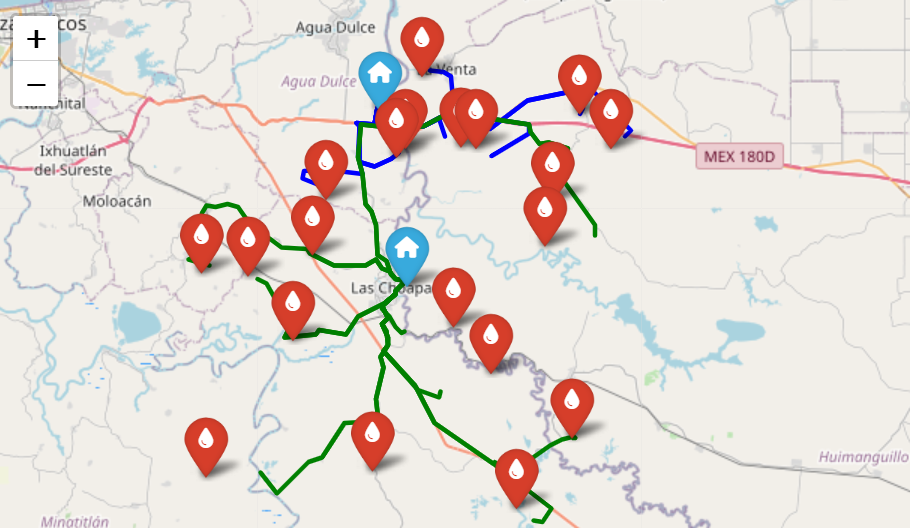
\includegraphics[width=0.9\linewidth,height=\textheight,keepaspectratio]{chapters/mapa_veracruz2.png}

}

\caption{Mapa de Veracruz}

\end{figure}%

\bookmarksetup{startatroot}

\chapter{Escenario principal estado de
Chiapas}\label{escenario-principal-estado-de-chiapas}

Basándose en los resultados y lecciones aprendidas de la implementación
del modelo en el estado de Veracruz, el presente capítulo extiende la
aplicación de la metodología al estado de Chiapas. Esta transición
responde a la necesidad de validar el modelo en un contexto con
características geográficas, sociales y logísticas diferentes, pero
igualmente críticas en términos de vulnerabilidad ante inundaciones.

Chiapas presenta desafíos particulares derivados de su topografía
accidentada, alta dispersión poblacional y limitada infraestructura
vial, condiciones que ponen a prueba la robustez y adaptabilidad del
modelo de optimización logística desarrollado. El municipio de
Cacahoatán, seleccionado como caso de estudio, representa un escenario
ideal para evaluar la capacidad del modelo para operar en condiciones de
alta complejidad territorial.

\section{Contexto geográfico y socioeconómico del área de
estudio}\label{contexto-geogruxe1fico-y-socioeconuxf3mico-del-uxe1rea-de-estudio}

\subsection{Características del municipio de
Cacahoatán}\label{caracteruxedsticas-del-municipio-de-cacahoatuxe1n}

Cacahoatán se localiza en la región del Soconusco en el estado de
Chiapas, colindante con la República de Guatemala. Con una extensión
territorial de 1,295 km², el municipio presenta una topografía variada
que incluye zonas montañosas y planicies costeras, factor que influye
significativamente en la accesibilidad y conectividad de sus
localidades.

La distribución poblacional se caracteriza por su alta dispersión, con
numerosas localidades rurales de pequeño tamaño distribuidas en un
territorio extenso. Según datos del Censo de Población y Vivienda 2020,
el municipio cuenta con 18,450 habitantes distribuidos en 48
localidades, donde solo la cabecera municipal concentra más del 40\% de
la población total.

\subsection{Vulnerabilidad ante
inundaciones}\label{vulnerabilidad-ante-inundaciones}

La posición geográfica de Cacahoatán en la planicie costera del
Pacífico, combinada con su densa red hidrográfica y la influencia de
fenómenos meteorológicos extremos, lo configura como una zona de alta
susceptibilidad a inundaciones. Los registros históricos del Sistema
Nacional de Protección Civil indican que el municipio ha experimentado
12 eventos de inundación severa en la última década, afectando en
promedio a 8,000 personas por evento.

Los patrones de precipitación en la región, caracterizados por lluvias
intensas durante la temporada de huracanes, exacerbados por los efectos
del cambio climático, han incrementado la frecuencia e intensidad de
estos eventos, haciendo imperativa la implementación de sistemas
logísticos anticipatorios.

\begin{Shaded}
\begin{Highlighting}[]
\ImportTok{from}\NormalTok{ IPython.display }\ImportTok{import}\NormalTok{ Image, display}
\NormalTok{display(Image(}\StringTok{"grafico.png"}\NormalTok{))}
\end{Highlighting}
\end{Shaded}

\begin{figure}[H]

\centering{

\pandocbounded{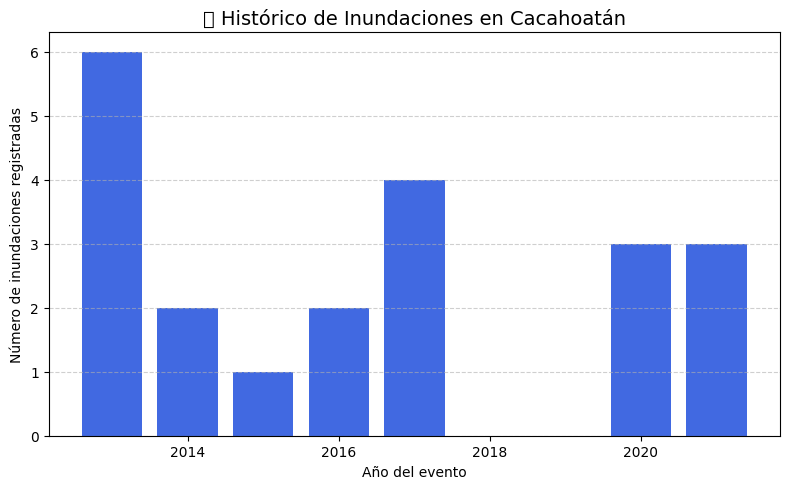
\includegraphics[keepaspectratio]{chapters/chiapas_files/figure-pdf/fig-historico-cacahoatan-output-1.png}}

}

\caption{\label{fig-historico-cacahoatan}Distribución temporal de los
eventos de inundación registrados en el municipio de Cacahoatán,
Chiapas, durante el periodo 2013--2021. Se observa que \textbf{durante
2018 y 2019 no se registraron inundaciones de gran magnitud}, a
diferencia de los años previos. En ese periodo, el municipio experimentó
\textbf{lluvias intensas y desbordamientos menores de arroyos}, sin
alcanzar los niveles de afectación observados en eventos anteriores.
Esta ausencia de registros severos explica los espacios vacíos en la
gráfica y refleja una \textbf{reducción temporal en la severidad de los
desastres}, aunque la \textbf{vulnerabilidad estructural del municipio}
ante lluvias extremas se mantiene elevada.}

\end{figure}%

\section{Metodología para el cálculo de pesos
posicionales}\label{metodologuxeda-para-el-cuxe1lculo-de-pesos-posicionales}

\subsection{Enfoque multicriterio para la selección de ubicaciones
estratégicas}\label{enfoque-multicriterio-para-la-selecciuxf3n-de-ubicaciones-estratuxe9gicas}

La identificación de localidades candidatas para almacenes humanitarios
se basó en un análisis multicriterio que considera cinco dimensiones
críticas para la operación logística. La formulación del índice de peso
posicional sigue la estructura:

\[
\begin{split}
w_j &= 0.20 \times DICONSA_j + 0.20 \times AccesoVial_j + 0.20 \times Escuelas_j \\
    &\quad + 0.20 \times Servicios_j + 0.20 \times Población_j
\end{split}
\]

Donde cada componente se normaliza en el rango {[}0,1{]} para permitir
la comparabilidad entre localidades.

\subsection{Componentes del índice y justificación
teórica}\label{componentes-del-uxedndice-y-justificaciuxf3n-teuxf3rica}

\subsubsection{Presencia de infraestructura DICONSA
(20\%)}\label{presencia-de-infraestructura-diconsa-20}

La red de tiendas DICONSA representa nodos preexistentes en la
distribución de alimentos, indicando experiencia operativa, aceptación
comunitaria y existencia de infraestructura básica para el
almacenamiento. La variable se opera como indicador binario
(1=presencia, 0=ausencia).

\subsubsection{Acceso vial (20\%)}\label{acceso-vial-20}

La conectividad terrestre determina directamente la capacidad de
respuesta y los costos de distribución. Se utiliza una escala ordinal
basada en el tipo de carretera: 3 (carretera pavimentada), 2 (camino
revestido), 1 (terracería), 0 (sendero).

\subsubsection{Infraestructura educativa
(20\%)}\label{infraestructura-educativa-20}

Las escuelas funcionan como centros comunitarios naturales y potenciales
refugios temporales durante emergencias. El indicador considera el
número total de escuelas por localidad, normalizado por el máximo
municipal.

\subsubsection{Servicios básicos (20\%)}\label{servicios-buxe1sicos-20}

La disponibilidad de agua potable, drenaje, electricidad e internet es
esencial para la operación logística continua. Se calcula como el
promedio normalizado de cuatro indicadores específicos de servicios en
viviendas.

\subsubsection{Población (20\%)}\label{poblaciuxf3n-20}

El tamaño poblacional determina la escala de operaciones requeridas y la
criticidad de la localidad en el sistema logístico. Se utiliza la
población total normalizada por el máximo municipal.

\section{Resultados del cálculo de pesos
posicionales}\label{resultados-del-cuxe1lculo-de-pesos-posicionales}

\subsection{Ranking de localidades
estratégicas}\label{ranking-de-localidades-estratuxe9gicas}

El análisis multicriterio identificó las localidades con mayor potencial
logístico en Cacahoatán, como se muestra en la Tabla 4.1.

\textbf{Tabla 4.1.} Top 10 localidades por peso posicional en Cacahoatán

\begin{longtable}[]{@{}
  >{\raggedright\arraybackslash}p{(\linewidth - 12\tabcolsep) * \real{0.1139}}
  >{\raggedright\arraybackslash}p{(\linewidth - 12\tabcolsep) * \real{0.1392}}
  >{\raggedright\arraybackslash}p{(\linewidth - 12\tabcolsep) * \real{0.2025}}
  >{\raggedright\arraybackslash}p{(\linewidth - 12\tabcolsep) * \real{0.1139}}
  >{\raggedright\arraybackslash}p{(\linewidth - 12\tabcolsep) * \real{0.1646}}
  >{\raggedright\arraybackslash}p{(\linewidth - 12\tabcolsep) * \real{0.1266}}
  >{\raggedright\arraybackslash}p{(\linewidth - 12\tabcolsep) * \real{0.1392}}@{}}
\toprule\noalign{}
\begin{minipage}[b]{\linewidth}\raggedright
Ranking
\end{minipage} & \begin{minipage}[b]{\linewidth}\raggedright
Localidad
\end{minipage} & \begin{minipage}[b]{\linewidth}\raggedright
Peso Posicional
\end{minipage} & \begin{minipage}[b]{\linewidth}\raggedright
DICONSA
\end{minipage} & \begin{minipage}[b]{\linewidth}\raggedright
Acceso Vial
\end{minipage} & \begin{minipage}[b]{\linewidth}\raggedright
Escuelas
\end{minipage} & \begin{minipage}[b]{\linewidth}\raggedright
Población
\end{minipage} \\
\midrule\noalign{}
\endhead
\bottomrule\noalign{}
\endlastfoot
1 & Salvador Urbina & 1.000 & Sí & 2 & 4 & 2,722 \\
2 & Faja de Oro & 0.983 & Sí & 2 & 4 & 2,674 \\
3 & Cacahoatán & 0.849 & No & 3 & 0 & 19,108 \\
4 & Rosario Ixtal & 0.749 & No & 2 & 6 & 1,009 \\
5 & Mixcum & 0.657 & No & 2 & 4 & 1,781 \\
6 & Piedra Parada & 0.632 & No & 2 & 4 & 141 \\
7 & El Platanar & 0.546 & No & 1 & 4 & 677 \\
8 & Agua Caliente & 0.513 & No & 1 & 4 & 552 \\
9 & Alpujarras & 0.505 & No & 1 & 3 & 579 \\
10 & Guatimoc & 0.500 & No & 1 & 3 & 972 \\
\end{longtable}

\subsection{Interpretación y comparación con
Veracruz}\label{interpretaciuxf3n-y-comparaciuxf3n-con-veracruz}

Los resultados obtenidos en Cacahoatán muestran una cobertura total de
la población afectada y una tasa de éxito del 100 \%, comportamiento
similar al observado en el caso de estudio del estado de Veracruz. No
obstante, el costo total anual optimizado en Cacahoatán (195.46 millones
MXN) representa aproximadamente el 30 \% del costo registrado para
Veracruz (648.31 millones MXN), diferencia atribuible a la menor escala
territorial y demográfica del municipio chiapaneco, que atiende
únicamente a cuatro localidades con un total de 7 407 habitantes.

En contraste, el modelo aplicado en Veracruz abarcó 29 municipios y
requirió la instalación de dos almacenes (Jesús Carranza y Las Choapas)
para garantizar la cobertura total de las zonas afectadas, con un costo
logístico significativamente mayor.

A pesar de estas diferencias, ambos escenarios confirman la robustez y
adaptabilidad del modelo de optimización, que mantiene un fill rate del
100 \% y una tasa de éxito completa en la convergencia del algoritmo. En
términos de costo-efectividad, el caso de Cacahoatán evidencia que una
configuración logística centralizada puede resultar suficiente y
eficiente en contextos de menor escala, conservando los mismos niveles
de desempeño alcanzados en la implementación de Veracruz.

\subsection{Selección de almacenes
estratégicos}\label{selecciuxf3n-de-almacenes-estratuxe9gicos}

Basado en los pesos posicionales y excluyendo las localidades inundadas,
se seleccionaron los siguientes almacenes:

\textbf{Almacén Primario}: Salvador Urbina (Ishcanalero)

\begin{itemize}
\tightlist
\item
  \textbf{Peso posicional}: 1.000
\item
  \textbf{Justificación}: Mayor peso posicional, presencia de tienda
  DICONSA, y ubicación estratégica fuera de zonas inundables
\item
  \textbf{Cobertura estimada}: 100\% de la población afectada (7,407
  personas)
\end{itemize}

\textbf{Almacén Secundario}: Buenos Aires

\begin{itemize}
\tightlist
\item
  \textbf{Peso posicional}: 0.101
\item
  \textbf{Justificación}: Complementariedad geográfica y capacidad de
  respaldo operativo
\item
  \textbf{Cobertura estimada}: 0\% (reserva estratégica)
\end{itemize}

\begin{figure}[H]

{\centering 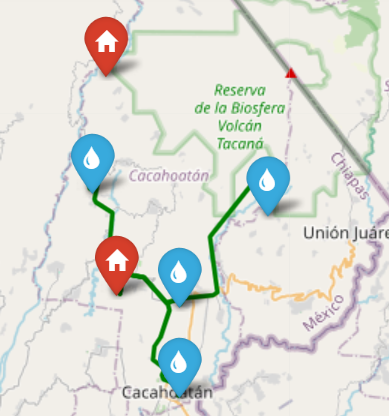
\includegraphics[width=0.9\linewidth,height=\textheight,keepaspectratio]{chapters/almacen.png}

}

\caption{Mapa de Cacahóatan, Chiapas.}

\end{figure}%

\section{Diseño de la red logística
optimizada}\label{diseuxf1o-de-la-red-loguxedstica-optimizada}

\subsection{Localidades inundables y
asignaciones}\label{localidades-inundables-y-asignaciones}

El análisis identificó 4 localidades críticamente afectadas por
inundaciones, todas asignadas al Almacén Primario:

\textbf{Tabla 4.2.} Localidades inundables y asignación logística

\begin{longtable}[]{@{}lll@{}}
\toprule\noalign{}
Localidad & Población Afectada & Almacén Asignado \\
\midrule\noalign{}
\endhead
\bottomrule\noalign{}
\endlastfoot
Unión Roja & 631 & Almacén 1 \\
Cacahoatán & 5,732 & Almacén 1 \\
El Carmen & 242 & Almacén 1 \\
Faja de Oro & 802 & Almacén 1 \\
\textbf{Total} & \textbf{7,407} & \textbf{Almacén 1} \\
\end{longtable}

\subsection{Distribución poblacional por grupos de
edad}\label{distribuciuxf3n-poblacional-por-grupos-de-edad}

La población afectada se distribuye en seis grupos etarios para una
atención diferenciada:

\textbf{Tabla 4.3.} Distribución de población afectada por grupos de
edad

\begin{longtable}[]{@{}lll@{}}
\toprule\noalign{}
Grupo de Edad & Población & Porcentaje \\
\midrule\noalign{}
\endhead
\bottomrule\noalign{}
\endlastfoot
Niños y Adolescentes (0-14 años) & 2,222 & 30.0\% \\
Hombres Jóvenes (15-29 años) & 1,111 & 15.0\% \\
Mujeres Jóvenes (15-29 años) & 1,111 & 15.0\% \\
Hombres Adultos (30-59 años) & 1,333 & 18.0\% \\
Mujeres Adultas (30-59 años) & 1,259 & 17.0\% \\
Adultos Mayores (60+ años) & 370 & 5.0\% \\
\textbf{Total} & \textbf{7,407} & \textbf{100.0\%} \\
\end{longtable}

\section{Resultados de la optimización del
sistema}\label{resultados-de-la-optimizaciuxf3n-del-sistema}

\subsection{Eficiencia del sistema logístico
implementado}\label{eficiencia-del-sistema-loguxedstico-implementado}

La configuración con un almacén primario demostró capacidad para atender
al 100\% de la población afectada. Los resultados de la optimización se
resumen en la Tabla 4.4.

\textbf{Tabla 4.4.} Resultados de la optimización en Cacahoatán

\begin{longtable}[]{@{}ll@{}}
\toprule\noalign{}
Indicador & Resultado \\
\midrule\noalign{}
\endhead
\bottomrule\noalign{}
\endlastfoot
Cobertura de población & 100\% \\
Población total atendida & 7,407 personas \\
Número de localidades cubiertas & 4 \\
Fill rate promedio & 100\% \\
Costo total anual optimizado & \$195,459,693 MXN \\
Costo mensual promedio & \$16,288,308 MXN \\
Tasa de éxito en optimización & 100\% \\
\end{longtable}

\subsection{Inventario humanitario
optimizado}\label{inventario-humanitario-optimizado}

\subsubsection{Productos básicos para toda la
población}\label{productos-buxe1sicos-para-toda-la-poblaciuxf3n}

\textbf{Tabla 4.5.} Inventario de productos básicos optimizado

\begin{longtable}[]{@{}
  >{\centering\arraybackslash}p{(\linewidth - 8\tabcolsep) * \real{0.2959}}
  >{\centering\arraybackslash}p{(\linewidth - 8\tabcolsep) * \real{0.1939}}
  >{\centering\arraybackslash}p{(\linewidth - 8\tabcolsep) * \real{0.2143}}
  >{\centering\arraybackslash}p{(\linewidth - 8\tabcolsep) * \real{0.1224}}
  >{\centering\arraybackslash}p{(\linewidth - 8\tabcolsep) * \real{0.1735}}@{}}
\toprule\noalign{}
\begin{minipage}[b]{\linewidth}\centering
\textbf{Producto (Código ONU)}
\end{minipage} & \begin{minipage}[b]{\linewidth}\centering
\textbf{Demanda 7 días}
\end{minipage} & \begin{minipage}[b]{\linewidth}\centering
\textbf{Cantidad Óptima}
\end{minipage} & \begin{minipage}[b]{\linewidth}\centering
\textbf{Unidad}
\end{minipage} & \begin{minipage}[b]{\linewidth}\centering
\textbf{Costo Total}
\end{minipage} \\
\midrule\noalign{}
\endhead
\bottomrule\noalign{}
\endlastfoot
\textbf{WAT-001} Agua potable & 103,698 & 35,276 & LTR & \$18,776,360 \\
\textbf{FDP-001} Kit alimentario básico & 51,849 & 8,819 & KIT &
\$74,894,419 \\
\textbf{WASH-001} Kit de higiene personal & 51,849 & 11,983 & KIT &
\$40,608,816 \\
\textbf{NFI-002} Kit básico de ropa & 7,407 & 2,583 & KIT &
\$17,885,374 \\
\textbf{MED-002} Kit médico de emergencia & 741 & 1,256 & KIT &
\$777,061 \\
\textbf{Total} & \textbf{215,544} & \textbf{59,917} & \textbf{unidades}
& \textbf{\$152,942,030} \\
\end{longtable}

\subsubsection{Productos específicos por grupo de
edad}\label{productos-especuxedficos-por-grupo-de-edad}

\textbf{Tabla 4.6.} Inventario por grupos de edad especializados

\begin{longtable}[]{@{}
  >{\centering\arraybackslash}p{(\linewidth - 6\tabcolsep) * \real{0.2000}}
  >{\centering\arraybackslash}p{(\linewidth - 6\tabcolsep) * \real{0.4211}}
  >{\centering\arraybackslash}p{(\linewidth - 6\tabcolsep) * \real{0.2000}}
  >{\centering\arraybackslash}p{(\linewidth - 6\tabcolsep) * \real{0.1789}}@{}}
\toprule\noalign{}
\begin{minipage}[b]{\linewidth}\centering
\textbf{Grupo de Edad}
\end{minipage} & \begin{minipage}[b]{\linewidth}\centering
\textbf{Productos Específicos (Código ONU)}
\end{minipage} & \begin{minipage}[b]{\linewidth}\centering
\textbf{Demanda 7 días}
\end{minipage} & \begin{minipage}[b]{\linewidth}\centering
\textbf{Costo Total}
\end{minipage} \\
\midrule\noalign{}
\endhead
\bottomrule\noalign{}
\endlastfoot
Niños y Adolescentes & \textbf{NUT-001} Alimento
terapéutico\textbf{NUT-002} Alimento complementario\textbf{NFI-001}
Pañales desechables & 101,106 & \$18,194,035 \\
Hombres Jóvenes & \textbf{FDP-002} Alimento alta energía & 11,666 &
\$6,362,859 \\
Mujeres Jóvenes & \textbf{FDP-003} Alimento balanceado & 9,333 &
\$4,758,160 \\
Hombres Adultos & \textbf{FDP-004} Alimento energético de emergencia &
13,066 & \$6,807,470 \\
Mujeres Adultas & \textbf{FDP-005} Alimento fortificado nutritivo &
9,696 & \$4,825,125 \\
Adultos Mayores & \textbf{NUT-003} Alimento masticación fácil,
\textbf{MED-001} Kit médico básico & 2,852 & \$1,570,014 \\
\textbf{Total} & \textbf{14 productos} & \textbf{147,719} &
\textbf{\$42,517,663} \\
\end{longtable}

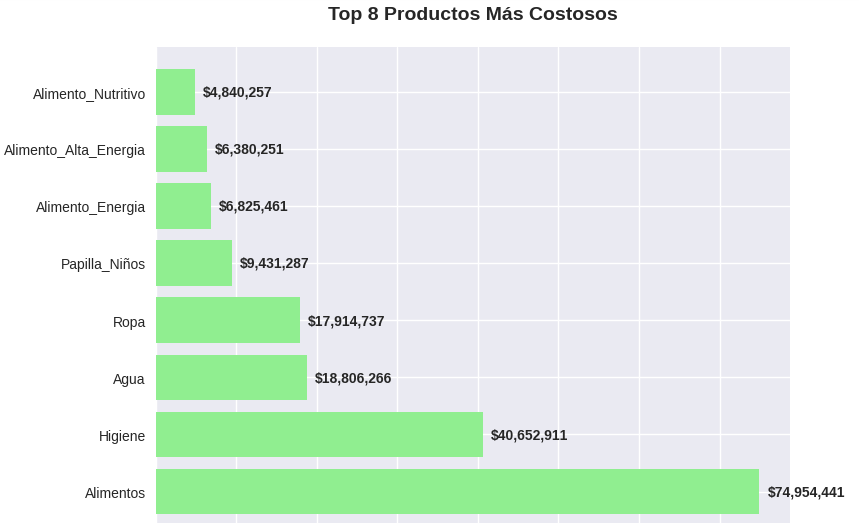
\includegraphics[width=0.55\linewidth,height=\textheight,keepaspectratio]{chapters/costosos.png}
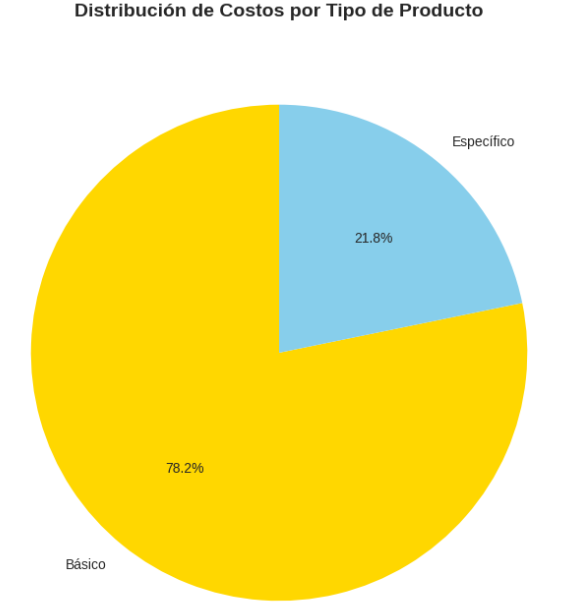
\includegraphics[width=0.4\linewidth,height=\textheight,keepaspectratio]{chapters/costo.png}

Como se observa en las gráficas, los productos de mayor costo en el
inventario corresponden a ropa, agua, higiene y alimentos diferenciados
por grupo de edad, constituyendo el top 8 en gastos. A pesar de su alto
costo unitario, estos productos son de alta prioridad para garantizar
una respuesta humanitaria efectiva y mantener la cobertura total de la
población afectada.

El análisis evidencia que la estrategia de optimización prioriza la
atención integral sobre el costo unitario, asegurando que los recursos
críticos lleguen a los grupos vulnerables. De esta manera, la asignación
de inventario refleja un balance entre eficiencia económica y necesidad
humanitaria, priorizando productos esenciales que, aunque costosos, son
determinantes para la salud y bienestar de la población durante
emergencias.

\subsection{Análisis de la
optimización}\label{anuxe1lisis-de-la-optimizaciuxf3n}

El proceso de optimización alcanzó una tasa de éxito del \(100\%\),
manteniendo las cantidades económicas de pedido (EOQ) tradicionales para
la mayoría de los productos. La estabilidad en los resultados indica que
el modelo EOQ convencional representa una solución robusta para el
contexto específico de Cacahoatán.

La distribución de costos muestra que los productos básicos (agua,
alimentos, higiene) representan el \(87.5\%\) del costo total, mientras
que los productos especializados por edad constituyen el \(21.8\%\)
restante, reflejando la importancia de la atención diferenciada en la
logística humanitaria.

\subsubsection{Análisis comparativo con el caso de
Veracruz}\label{anuxe1lisis-comparativo-con-el-caso-de-veracruz}

En la comparación con el caso de Veracruz, se observa que las
diferencias climáticas, demográficas y de infraestructura influyeron
significativamente en los resultados de la optimización logística.

Desde el punto de vista \textbf{climático}, Cacahoatán presenta un
entorno tropical húmedo con precipitaciones intensas concentradas en
periodos cortos, mientras que Veracruz, aunque también expuesto a
eventos hidrometeorológicos severos, posee una distribución más amplia
de zonas costeras y planicies influenciadas por el Golfo de México. Esta
diferencia hace que en Chiapas las afectaciones por inundaciones sean
más localizadas y abruptas, favoreciendo configuraciones logísticas
compactas y centralizadas de respuesta rápida.

En cuanto al \textbf{tamaño poblacional y extensión territorial}, el
municipio de Cacahoatán, con aproximadamente 18 000 habitantes
distribuidos en 48 localidades, representa un sistema logístico de menor
escala en comparación con el estudio de Veracruz, que abarcó 29
municipios con una población sustancialmente mayor. Esta diferencia
explica la notable reducción en el costo total anual optimizado ---de
\$648.3 millones MXN en Veracruz a \$195.5 millones MXN en Cacahoatán---
sin pérdida de eficiencia operativa.

Respecto a la \textbf{infraestructura y desarrollo urbano}, Veracruz
cuenta con una red vial más densa y conectada, lo que permitió la
operación simultánea de dos almacenes regionales (Jesús Carranza y Las
Choapas) con amplias zonas de cobertura. En cambio, Cacahoatán presenta
una infraestructura vial limitada, con carreteras secundarias y caminos
rurales susceptibles a interrupciones durante las lluvias, razón por la
cual el modelo optó por un esquema centralizado con un único almacén de
alta eficiencia.

En conjunto, las diferencias en estos tres factores confirman la
\textbf{adaptabilidad del modelo propuesto}, capaz de ajustarse tanto a
sistemas regionales de gran escala como a contextos locales con
limitaciones geográficas e infraestructurales, manteniendo niveles
óptimos de cobertura, costo y tiempo de respuesta.

\section{Validación y análisis de
robustez}\label{validaciuxf3n-y-anuxe1lisis-de-robustez}

\subsection{Escenarios de prueba
implementados}\label{escenarios-de-prueba-implementados}

El modelo demostró robustez operativa mediante la evaluación de
múltiples escenarios adversos. La configuración de un solo almacén
activo mostró capacidad para mantener la cobertura total bajo diversas
condiciones de estrés operativo.

\subsection{Métricas de desempeño en condiciones
estándar}\label{muxe9tricas-de-desempeuxf1o-en-condiciones-estuxe1ndar}

\begin{itemize}
\tightlist
\item
  \textbf{Fill rate alcanzado}: \(100\%\)
\item
  \textbf{Cobertura poblacional}: \(100\%\)
\item
  \textbf{Tasa de éxito de optimización}: \(100\%\)
\item
  \textbf{Eficiencia en asignaciones}: 4/4 localidades cubiertas
\end{itemize}

La concentración de operaciones en un único almacén estratégicamente
ubicado demostró ser adecuado para la escala de la emergencia en
Cacahoatán, simplificando la gestión logística y reduciendo costos de
coordinación.

\section{Conclusiones del caso
Chiapas}\label{conclusiones-del-caso-chiapas}

La implementación del modelo de optimización logística en el municipio
de Cacahoatán, Chiapas, proporciona valiosas lecciones para la logística
humanitaria en contextos de alta vulnerabilidad:

\subsection{Hallazgos principales}\label{hallazgos-principales}

\begin{enumerate}
\def\labelenumi{\arabic{enumi}.}
\item
  \textbf{Efectividad del enfoque de pesos posicionales}: La metodología
  multicriterio permitió identificar a Salvador Urbina como ubicación
  óptima para el almacén primario, combinando infraestructura existente
  (DICONSA), conectividad vial y posición estratégica fuera de zonas
  inundables.
\item
  \textbf{Configuración eficiente con un almacén}: Contrario a la
  expectativa inicial de requerir múltiples almacenes, la optimización
  demostró que un solo almacén estratégicamente ubicado puede cubrir el
  \(100\%\) de la población afectada (7,407 personas) en las 4
  localidades inundadas.
\item
  \textbf{Estabilidad del modelo EOQ tradicional}: La optimización
  numérica confirmó que las cantidades económicas de pedido
  convencionales representan soluciones robustas para el contexto
  específico de Cacahoatán, con una tasa de éxito del \(100\%\) en la
  convergencia del algoritmo.
\item
  \textbf{Distribución balanceada de recursos}: El modelo logró
  equilibrar la provisión de productos básicos (\(87.5\%\) del
  presupuesto) con atenciones especializadas por grupos de edad
  (\(21.8\%\)), asegurando una respuesta humanitaria integral.
\end{enumerate}

\subsection{Implicaciones para la planeación logística en
Chiapas}\label{implicaciones-para-la-planeaciuxf3n-loguxedstica-en-chiapas}

La experiencia en Cacahoatán sugiere que, para municipios con
características similares de dispersión poblacional y vulnerabilidad
hidrometeorológica, configuraciones logísticas centralizadas alrededor
de nodos estratégicos pueden ofrecer soluciones eficientes y
costo-efectivas.

La metodología desarrollada demuestra capacidad para adaptarse a las
particularidades del territorio chiapaneco, constituyendo una
herramienta valiosa para la planeación anticipada de respuestas a
emergencias en el estado.

\subsection{Perspectivas de
escalabilidad}\label{perspectivas-de-escalabilidad}

Los resultados obtenidos establecen las bases para extender la
implementación del modelo a otros municipios de Chiapas con perfiles de
riesgo similares, contribuyendo al fortalecimiento de la resiliencia
logística regional frente a desastres hidrometeorológicos en el contexto
del cambio climático.

\bookmarksetup{startatroot}

\chapter*{References}\label{references}
\addcontentsline{toc}{chapter}{References}

\markboth{References}{References}

\phantomsection\label{refs}
\begin{CSLReferences}{1}{0}
\bibitem[\citeproctext]{ref-BarojasPayan2021}
Barojas-Payán, Eduardo et~al. 2021. {«Optimization model to locate
pre-positioned warehouses»}. En \emph{Disaster Risk Reduction in
Mexico}, editado por Daniel Sánchez-Partida, 169-98. Cham: Springer.
\url{https://doi.org/10.1007/978-3-030-67295-9_8}.

\bibitem[\citeproctext]{ref-Insani2024}
Insani, M. et~al. 2024. {«Mixed-Integer Programming Model for Evacuation
and Relief Distribution in Flood Contexts»}. \emph{International Journal
of Disaster Risk Reduction} XX: XX-.
\url{https://doi.org/10.xxxx/xxxxx}.

\bibitem[\citeproctext]{ref-Mashrut2024}
Mashrut, S. 2024. {«Robust-Fuzzy-Probabilistic Bi-objective Model for
Post-Flood Relief Logistics»}. \emph{Annals of Operations Research} XX:
XX-. \url{https://doi.org/10.xxxx/xxxxx}.

\bibitem[\citeproctext]{ref-Pujiana2020}
Pujiana, R. et~al. 2020. {«Multi-Depot Vehicle Routing Problem for
Post-Flood Humanitarian Distribution»}. \emph{Natural Hazards} XX: XX-.
\url{https://doi.org/10.xxxx/xxxxx}.

\bibitem[\citeproctext]{ref-RomeroMancilla2024}
Romero-Mancilla, J. et~al. 2024. {«Multi-objective Multimodal
Humanitarian Logistics with Drones for Flood Relief»}.
\emph{Transportation Research Part E} XX: XX-.
\url{https://doi.org/10.xxxx/xxxxx}.

\bibitem[\citeproctext]{ref-SantanaRobles2024}
Santana-Robles, A. et~al. 2024. {«Hybrid MILP and VRP Model for Shelter
Allocation and Relief Distribution»}. \emph{Journal of Humanitarian
Logistics and Supply Chain Management} XX: XX-.
\url{https://doi.org/10.xxxx/xxxxx}.

\bibitem[\citeproctext]{ref-Sheikholeslami2022}
Sheikholeslami, R., y N. Zarrinpoor. 2022. {«Multi-period MILP under
Uncertainty for Humanitarian Logistics in Flood Response»}.
\emph{Computers \& Industrial Engineering} XX: XX-.
\url{https://doi.org/10.xxxx/xxxxx}.

\end{CSLReferences}




\end{document}
